\documentclass[mathserif]{beamer}
\usepackage{beamerthemeshadow}
\usepackage{beamerthemesplit}
%\usetheme{shadow}
\usecolortheme{default}
\setbeamertemplate{footline}[frame number]
\useinnertheme[shadow=true]{rounded}
%\setbeamertemplate{footline}{\insertframenumber/\inserttotalframenumber}
%\useoutertheme{infolines}
%\setbeamertemplate{headline}{} % removes the headline that infolines inserts

%\usetheme{boxes}
%\usepackage{amsmass}
%\usepackage{amssymb,amsfonts,url}


\usepackage{algorithm}
\usepackage{algorithmic}

\usepackage{graphicx}
\graphicspath{{Problems/}}
\usepackage{subfigure}


\usepackage{tikz}
\usetikzlibrary{shadows}
\usepackage{verbatim}
\usepackage{pgfplots}
\usepackage{verbatim}
\usetikzlibrary{arrows,shapes}

\definecolor{darkblue}{rgb}{0.2,0.2,0.6}
\definecolor{darkred}{rgb}{0.6,0.1,0.1}
\definecolor{darkgreen}{rgb}{0.2,0.6,0.2}

\usetikzlibrary{shadings,shadows,shapes.arrows}

\usetikzlibrary{calc} 
\makeatletter 
\@namedef{color@3}{blue!20}
\@namedef{color@1}{green!70}   
%\@namedef{color@3}{yellow!50} 
\@namedef{color@2}{orange!90}  
%\@namedef{color@5}{magenta!70} 
%\@namedef{color@6}{yellow!70}    

\newcommand{\graphitemize}[2]{%
\begin{tikzpicture}[every node/.style={align=center}, scale=0.78]  
 \draw[fill=green!5, fill opacity=0.1, green, inner sep=0.05cm, outer sep=0.05cm] (5,0) arc(0:360:5);
 % \draw[fill=white, fill opacity=0.1, white, inner sep=0.05cm, outer sep=0.05cm] (4,0) arc(0:360:4);
%  \shade[ball color=gray!10!] (0,0) coordinate(Hp) circle (.9);
  \node[shape=circle,  minimum size=1.1cm,fill=red!60,font=\Large,outer sep =.15cm,inner sep=.2cm,drop  shadow={ashadow, color=red!60!black}](ce){#1};  
   % \shade[ball color=blue!20!] (0,0) coordinate($Algorithm$) circle (1.5cm);

\foreach \gritem [count=\xi] in {#2}  {\global\let\maxgritem\xi}  
\foreach \gritem [count=\xi] in {#2}
{% 
\pgfmathtruncatemacro{\angle}{90+360/\maxgritem*\xi}
\edef\col{\@nameuse{color@\xi}}
\node[shape=circle,
     ultra thick,
     draw=white,
     fill opacity=1,
     drop  shadow={ashadow, color=blue!60},
     fill=\col,outer sep=0.25cm,        
     minimum size=2cm] (satellite-\xi) at (\angle:5cm) {\gritem };
     \draw[line width=0.25cm,-latex, \col] (ce) -- (satellite-\xi);
     }%
% \draw[violet, fill=violet!10] (4,0) arc(0:360:4);
\end{tikzpicture}  
}%



\newcommand*{\tikzarrow}[2]{%
  \tikz[
    baseline=(A.base),             % Set baseline to the baseline of node content
    font=\footnotesize\sffamily    % Set fontsize of the node content
  ]
  \node[
    single arrow,                  % Shape of the node
    single arrow head extend=2pt,  % Actual width of arrow head
    draw,                          % Draw the node shape
    inner sep=2pt,                 % Separation between node content and node shape
    top color=white,               % Shading color on top of node
    bottom color=#1,               % Shading color on bottom of node
    drop shadow                    % Draw a shadow
  ] (A) {#2};%
}


\def\arrow{
  (10.05:1.1) -- (6.05:1) arc (6.05:120:1) [rounded corners=0.5] --
  (120:0.9) [rounded corners=1] -- (130:1.1) [rounded corners=0.5] --
  (120:1.3) [sharp corners] -- (120:1.2) arc (120:5.25:1.2)
  [rounded corners=1] -- (10.05:1.1) -- (6.05:1) -- cycle
}

\tikzset{
  ashadow/.style={opacity=.25, shadow xshift=0.07, shadow yshift=-0.07},
}

\def\arrows[#1]{         
  \begin{scope}[scale=#1]
    \draw[color=darkred, drop  shadow={ashadow, color=red!60!black}] \arrow;

    \draw[color=darkgreen, bottom color=green!90!black, top color=green!60,   drop shadow={ashadow, color=green!60!black}] [rotate=120] \arrow;

    \draw[color=darkblue, right color=blue, left color=blue!60,   drop shadow={ashadow, color=blue!60!black}] [rotate=240] \arrow;

    % to hide the green shadow
    \draw[color=darkred, left color=red, right color=red!60] \arrow;
  \end{scope}
}

\tikzstyle{vertex}=[circle,fill=black!25,draw,minimum size=20pt,inner sep=0pt]
\tikzstyle{smallvertex}=[circle,fill=black!25,draw,minimum size=10pt,inner sep=0pt]
\tikzstyle{selected vertex} = [vertex, draw,fill=red!24]
\tikzstyle{blue smallvertex} = [smallvertex, draw,fill=blue]
\tikzstyle{red smallvertex} = [smallvertex, draw,fill=red]
\tikzstyle{edge} = [draw,thick,->]
\tikzstyle{undirectededge} = [draw,thick]
\tikzstyle{weight} = [font=\small]
\tikzstyle{selected edge} = [draw,line width=5pt,-,red!50]
\tikzstyle{ignored edge} = [draw,line width=5pt,-,black!20]



\title{CS711008Z  Algorithm Design and Analysis }
\subtitle{ Lecture 1. Introduction and some representative problems
\footnote{The slides are made based on Chapter 1 of Algorithm design. Some slides are excerpted from Kevin Wayne's slides with permission. } 
}
\author{Dongbo Bu \\
\ \ \ \ \ \ \ \ \ \ \ \ \ \ \ \ \ \ \ \ \ \ \ \ \ \ \ \ \ \ \ \ \ \ \ \ \ \ \ \ \ \ \ \ \ \ \ \ \ \ \ \ \ \ \ \ \ \ \ \ \ \ \ \ \ \ \ \ \ \ \ \ \ \ \ \ \ \ \ \ \ \ \ \ \ \ \ \ \ \ \ \ \ \ \ \ \ \ \ \  \\
{\small Institute of Computing Technology \\ Chinese Academy of Sciences, Beijing, China}}
\date{}


\begin{document}
%\begin{CJK}{UTF8}{cyberbit}

\frame{\titlepage}

%\section[Outline]{}
%\frame{\tableofcontents}

%    \begin{figure}
%        \centering
%        \includegraphics[width=0.8\textwidth]{newGeneRep.eps}
%    \end{figure}

% \begin{figure}%
%   \begin{center}%
%     \begin{minipage}{0.70\textwidth}%
%      \includegraphics[width=1.0\textwidth]{comp25000.eps}%
%     \end{minipage}%
%     \begin{minipage}{0.30\textwidth}
%      \includegraphics[width=1.0\textwidth]{comparelabel.eps}%
%     \end{minipage}%
%   \end{center}
% \end{figure}

% \begin{table}
%   {\begin{tabular}{l|rrr}\hline
%       & \multicolumn{3}{c}{Actual number of DCJ operations}\\
%       \# genes &\# genes $\times 1$&\# genes $\times 2$&\# genes  $\times 3$ \\
% \hline
%      (a)~25,000 & 0.5\% ~~&  0.9\% ~~& 1.7\%~~\\
%       (b)~10,000 & 0.8\%~~ &  1.4\% ~~& 2.7\%~~\\
%      (c)~ 1,000 & 2.7\%~~ & 4.7\%~~ & 14.7\%~~\\ \hline
%     \end{tabular}} {}%
% \end{table}

\frame{
%\frametitle{Algorithm}

\begin{block}{}
 
 {\bf Algorithm design: the art of computer programming }
\end{block}

    \begin{figure}
        \centering
        
\includegraphics[width=0.4\textwidth]{L1-The-Art.jpg}
    \end{figure}
}

\frame{
\frametitle{V. Vazirani said: }

\begin{block}{}
{\it  Our philosophy on the design and exposition of algorithms is nicely illustrated by the following analogy with an aspect of Michelangelos's art:  \\
A major part of his effort involved looking for interesting pieces of stone in the quarry and staring at them for long hours \textcolor{red}{to determine the form they naturally wanted to take}. The chisel work exposed, in a minimal manner, this form. \\ 
}
\end{block}
    \begin{figure}
        \centering
        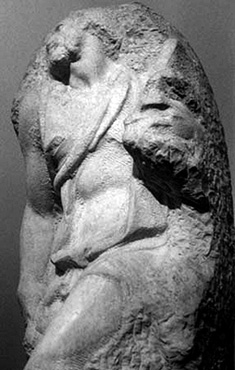
\includegraphics[width=2in]{L1-unfinished.jpg}
    \end{figure}
}

\frame{
\frametitle{V. Vazirani said:  $cont'd$ }

\begin{block}{}
{\it By analogy, we would like to start with a clean, simply stated problem. \\
Most of the algorithm design effort actually goes into \textcolor{red}{understanding the algorithmically relevant combinatorial structure of the problem}. \\
The algorithm exploits this structure in a minimal manner..... \\
with emphasis on stating the structure offered by the problems, and keeping the algorithms minimal.  }
\end{block}

(See two extra slides.)
}

%  \frame {
%  \frametitle{A first problem: Regular expression matching problem}
%  Contributed by Yanbing Liu, Security lab at ICT. \\
%  (see extra slides.)
%  }
 
% \frame {
% \frametitle{A first problem: Regular expression matching problem}
% \begin{itemize}
%  \item Key observation: solution=vector;
%  \item Solution space size: $O(\prod_{i=1}^n \mid S_i \mid)$ %$O(prod_{i=1}^n S_i)$
%  \item Brute-force: $O(\prod_{i=1}^n \mid S_i \mid)$ time. 
% \end{itemize}
% 
% \begin{figure}
%         \centering
%         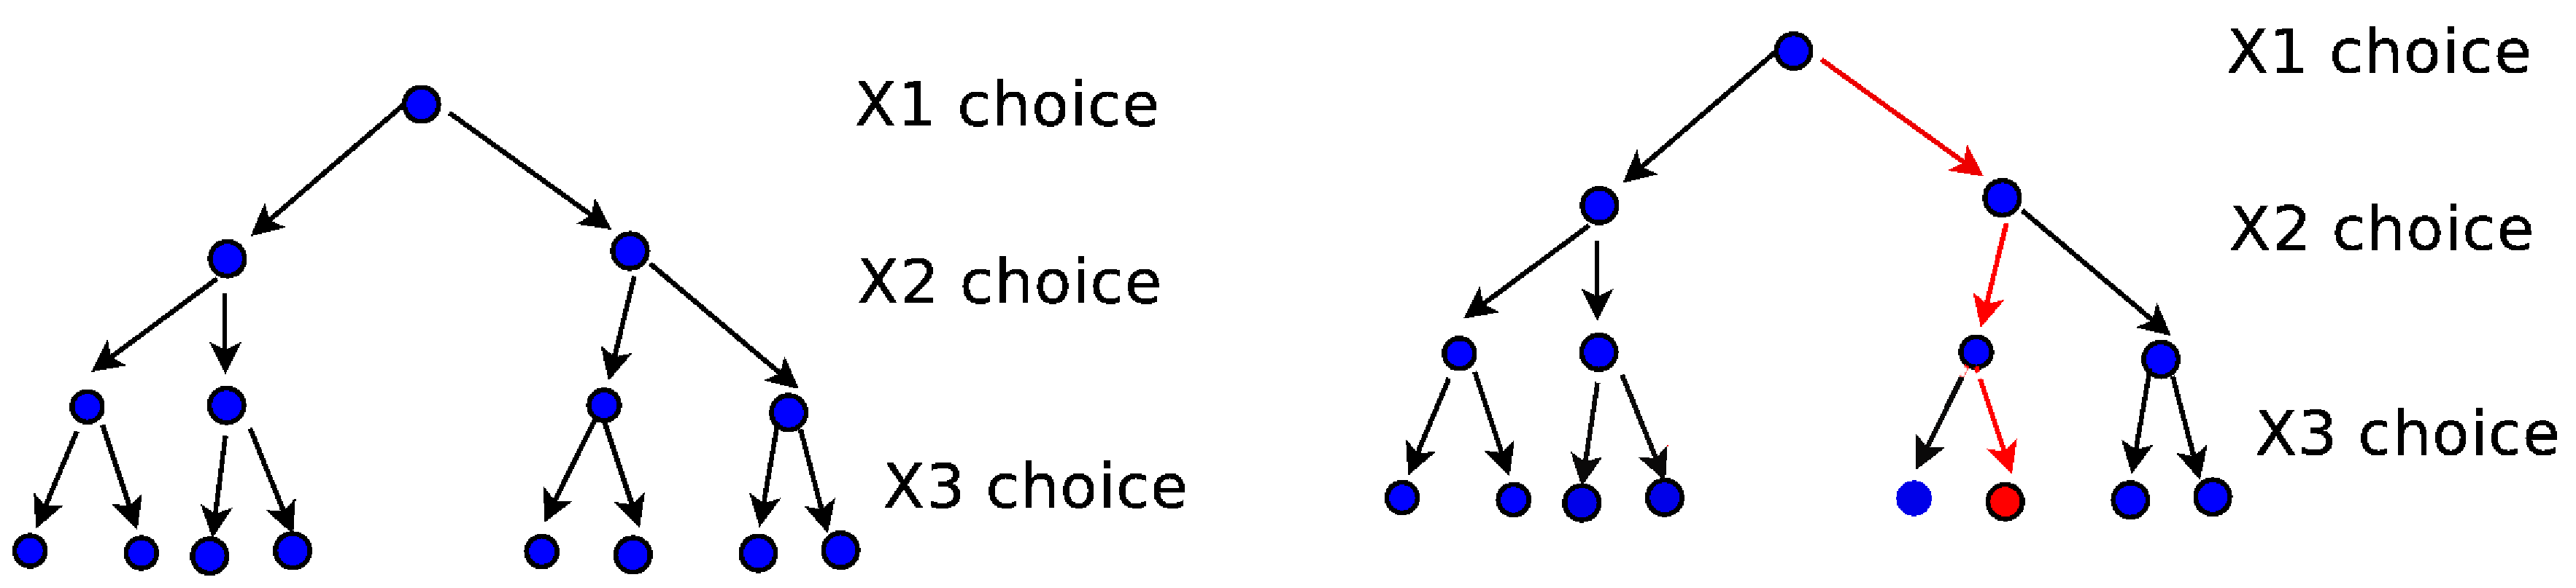
\includegraphics[width=4in]{L1-regularexpressionsearchspace.eps}
% \end{figure}
% }
% 
% 
% \frame {
% \frametitle{A first problem: Regular expression matching problem  $(cont'd)$ }
% \begin{itemize}
%  \item 
% Key observation: solution=vector=path; solution can be decomposed. \\
% \item Key idea: run BFS to check whether the final nodes are reachable; or dynamic programming;
% \item Time-complexity:  $O(4*n)$ \\
% \end{itemize}
% 
% \begin{figure}
%         \centering
%         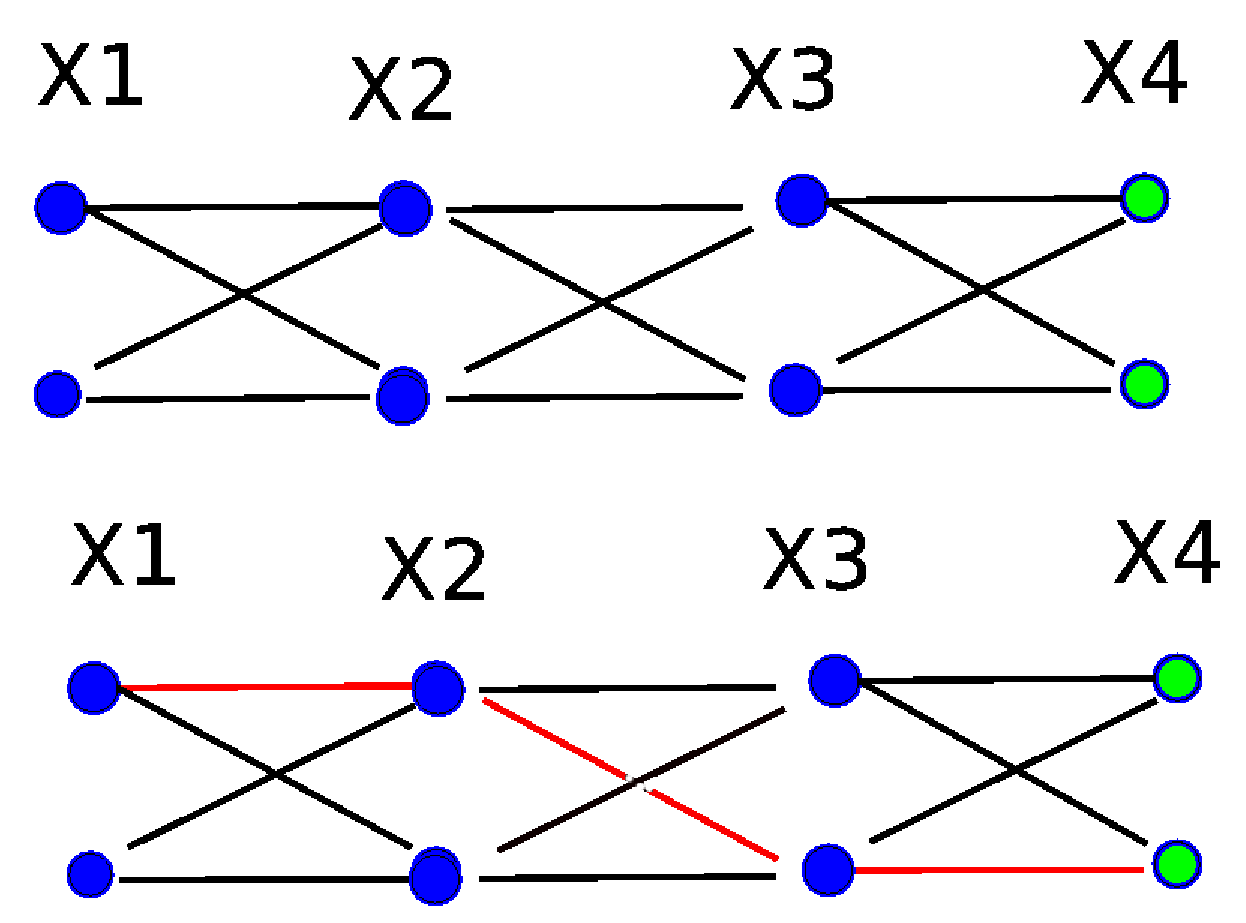
\includegraphics[width=2in]{L1-regularexpressionalgo.eps}
% \end{figure}
% 
%}



\frame {
 \frametitle{The first problem: {\sc Stable Matching} problem}
 \begin{itemize}
 \item 
In 1962, David Gale and Lloyd Shapley asked a question: Could one design a college admissions process, or a job recruiting process that is self-enforcing? 
\item 
\textcolor{blue}{ {\bf 
Motivation: } } Consider some students applying to company for internships. 
\begin{itemize}
     \item Raj accepted an offer from CluNet company;
     \item WebExodus offers Raj a summer job later;
     \item Raj retract his acceptance of the CluNet offer;
     \item CluNet has to offer a jobs to one of his wait-listed applicants;
     \item This applicant retracts his acceptance to a company BabelSoft;
     \item ......
    \end{itemize}
\end{itemize}
}

\frame
{
\frametitle{{\sc Stable Matching} -- Problem Statement}
In mathematics, the {\sc Stable Matching}  problem is the problem of
finding a stable matching --- a matching in which two agents cannot be found who would prefer each other over their current counterparts.
\begin{block}{Formalization:}
{\bf Input:}\\
$n$ men and $n$ women, where each person has ranked all members of the opposite
sex with a unique number between $1$ and $n$ in order of preference.

{\bf Output:}\\
A matching of the men and women such that there is no \textcolor{blue}{unstable pair}.
\end{block}
}

\frame{
\frametitle{Two men and two women: unstable matching}
\begin{itemize}
\item 
 Example 1: (consensus preference: 1 stable matching) \\ 
       $m$ prefers $w$ to $w'$; \\
       $m'$ prefers $w$ to $w'$; \\
       $w$ prefers $m$ to $m'$; \\
       $w'$ prefers $m$ to $m'$; \\
       
\begin{figure}
\begin{tikzpicture}[scale=1.1, auto,swap]
    % Draw a 7,11 network
    % First we draw the vertices
    \foreach \pos/ \name in {{(0,0)/m'},{(0,1.5)/m}} 
        \node[vertex,fill=blue!20] (\name) at \pos{$\name$};

    \foreach \pos/\name in {{(2,0)/w'}, {(2,1.5)/w}}
        \node[vertex,fill=green] (\name) at \pos {$\name$};
     
    % Connect vertices with edges and draw weights
    \foreach \source/ \dest/\weight in {m/w/{}, m'/w'/{} }
        \path[undirectededge] (\source) -- node[weight] {$\weight$} (\dest);
%       \draw[dashed, ->] (0,0) arc  (120:60:2);

   \node[above] at (1, 2 ) {Match $1$}; 
   
   
   
   
       \foreach \pos/ \name in {{(4,0)/m'},{(4,1.5)/m}} 
        \node[vertex,fill=blue!20] (\name) at \pos{$\name$};

    \foreach \pos/\name in {{(6,0)/w'}, {(6,1.5)/w}}
        \node[vertex,fill=green] (\name) at \pos {$\name$};
     
    % Connect vertices with edges and draw weights
    \foreach \source/ \dest/\weight in {m/w'/{}, m'/w/{} }
        \path[undirectededge] (\source) -- node[weight] {$\weight$} (\dest);
%       \draw[dashed, ->] (0,0) arc  (120:60:2);

   \foreach \source/ \dest/\weight in {m/w/{}}
        \path[undirectededge, red, dashed] (\source) -- node[weight] {$\weight$} (\dest);


   \node[above] at (5, 2 ) {Match $2$}; 
   
   
   
      \end{tikzpicture}

\end{figure}

\item In matching 2, $m$ and $w$ form an \textcolor{red}{\tt unstable pair:} (red, dashed line)\\
--- both $m$ and $w$ prefer the other to their current partners;
\end{itemize}
}

\frame{
\frametitle{Two men and two women: stable matching}
\begin{itemize}
\item 
Example 2: (different preference: 2 stable matchings) \\
       $m$ prefers $w$ to $w'$; \\
       $m'$ prefers $w'$ to $w$; \\
       $w$ prefers $m'$ to $m$; \\
       $w'$ prefers $m$ to $m'$;  \\
\begin{figure}
\begin{tikzpicture}[scale=1.1, auto,swap]
    % Draw a 7,11 network
    % First we draw the vertices
    \foreach \pos/ \name in {{(0,0)/m'},{(0,1.5)/m}} 
        \node[vertex,fill=blue!20] (\name) at \pos{$\name$};

    \foreach \pos/\name in {{(2,0)/w'}, {(2,1.5)/w}}
        \node[vertex,fill=green] (\name) at \pos {$\name$};
     
    % Connect vertices with edges and draw weights
    \foreach \source/ \dest/\weight in {m/w/{}, m'/w'/{} }
        \path[undirectededge] (\source) -- node[weight] {$\weight$} (\dest);
%       \draw[dashed, ->] (0,0) arc  (120:60:2);

   \node[above] at (1, 2 ) {Match $1$}; 
   
   
   
   
       \foreach \pos/ \name in {{(4,0)/m'},{(4,1.5)/m}} 
        \node[vertex,fill=blue!20] (\name) at \pos{$\name$};

    \foreach \pos/\name in {{(6,0)/w'}, {(6,1.5)/w}}
        \node[vertex,fill=green] (\name) at \pos {$\name$};
     
    % Connect vertices with edges and draw weights
    \foreach \source/ \dest/\weight in {m/w'/{}, m'/w/{} }
        \path[undirectededge] (\source) -- node[weight] {$\weight$} (\dest);
%       \draw[dashed, ->] (0,0) arc  (120:60:2);

%   \foreach \source/ \dest/\weight in {m/w/{}}
%        \path[undirectededge, red, dashed] (\source) -- node[weight] {$\weight$} (\dest);


   \node[above] at (5, 2 ) {Match $2$}; 
   
   
   
      \end{tikzpicture}

\end{figure}

\item Both matching 1 and 2 are stable.
\end{itemize}
}


% \frame{
% \frametitle{unstable match}
% 
% {\bf $m$ and $w'$ are unstable match:} \\
% --- both $m$ and $w'$ prefer the other to their current partnets;
% 
%     \begin{figure}
%         \centering
%         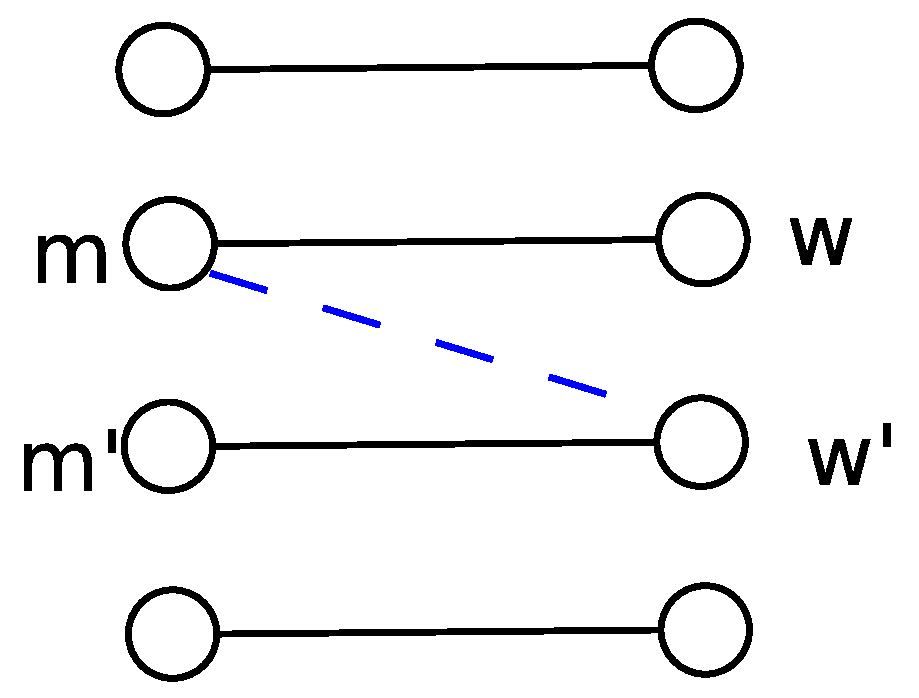
\includegraphics[width=0.8\textwidth]{unstable.eps}
%     \end{figure}
% 
% }


\frame{
\frametitle{Three men and three women: unstable matching}
\begin{figure}
 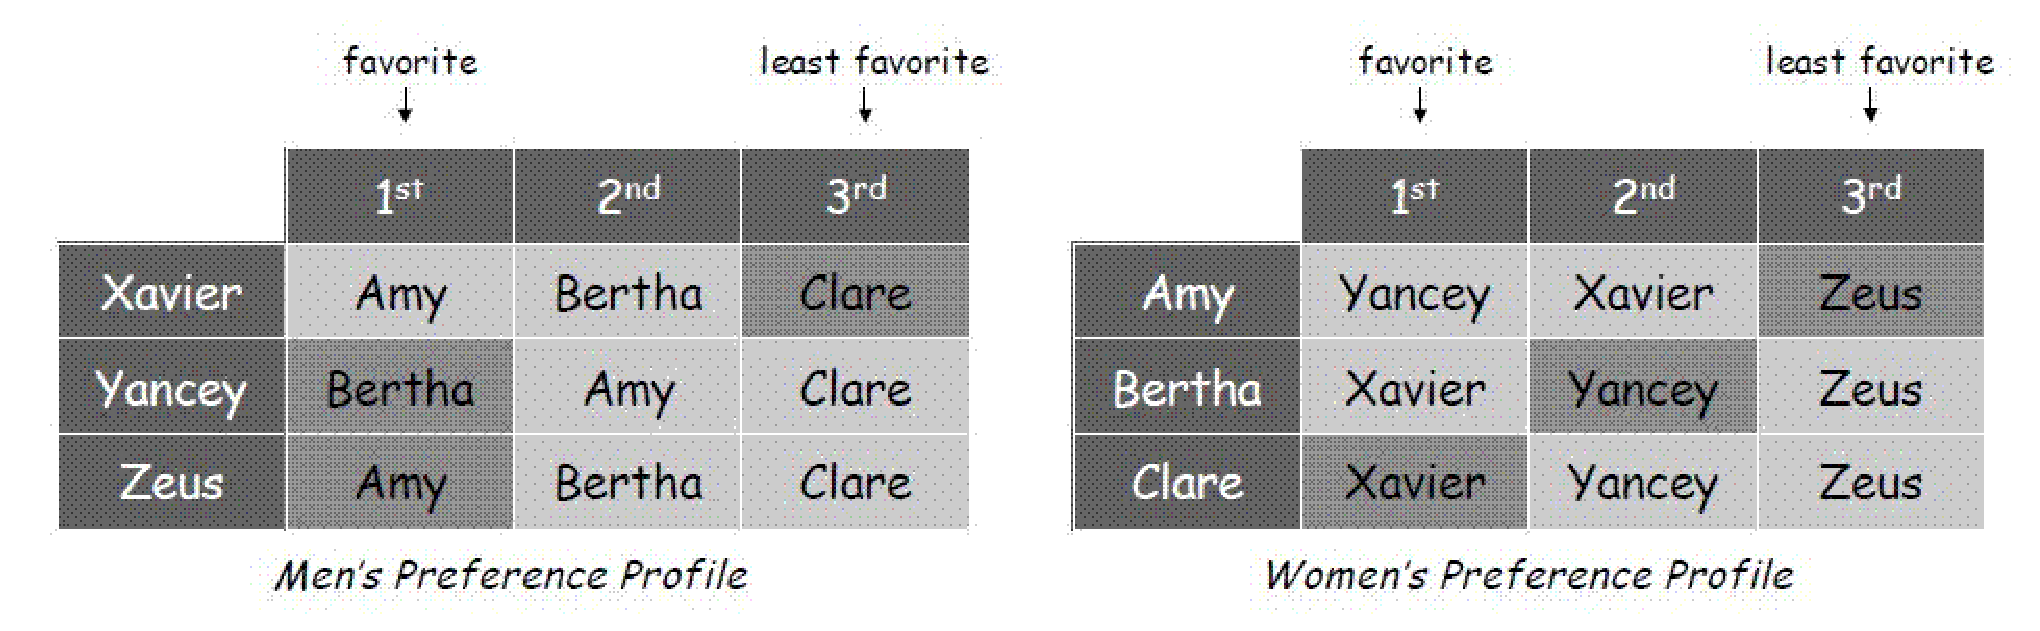
\includegraphics[width=4in] {L1-unstablematchingexampleXYZABC.eps}
\end{figure}
\begin{itemize}
 \item 
Is matching $X-C,\ Y-B,\ Z-A$ stable? \\
\item 
No. Bertha and Xavier will hook up. 
\end{itemize}
\begin{figure}
\begin{tikzpicture}[scale=0.8, auto,swap]
    % Draw a 7,11 network
    % First we draw the vertices
    \foreach \pos/ \name in {{(0,0)/Z},{(0,1.5)/Y},{(0,3)/X}} 
        \node[vertex,fill=blue!20] (\name) at \pos{$\name$};

    \foreach \pos/ \name in {{(3.6,0)/C},{(3.6,1.5)/B},{(3.6,3)/A}} 
        \node[vertex,fill=green] (\name) at \pos {$\name$};
     
    % Connect vertices with edges and draw weights
    \foreach \source/ \dest/\weight in {X/C/{}, Y/B/{}, Z/A/{} }
        \path[undirectededge] (\source) -- node[weight] {$\weight$} (\dest);
%       \draw[dashed, ->] (0,0) arc  (120:60:2);

   \foreach \source/ \dest/\weight in {X/B/{}}
        \path[undirectededge, red, dashed] (\source) -- node[weight] {$\weight$} (\dest);


      \end{tikzpicture}

\end{figure}


}

\frame{
\frametitle{Three men and three women: stable matching}
\begin{figure}
 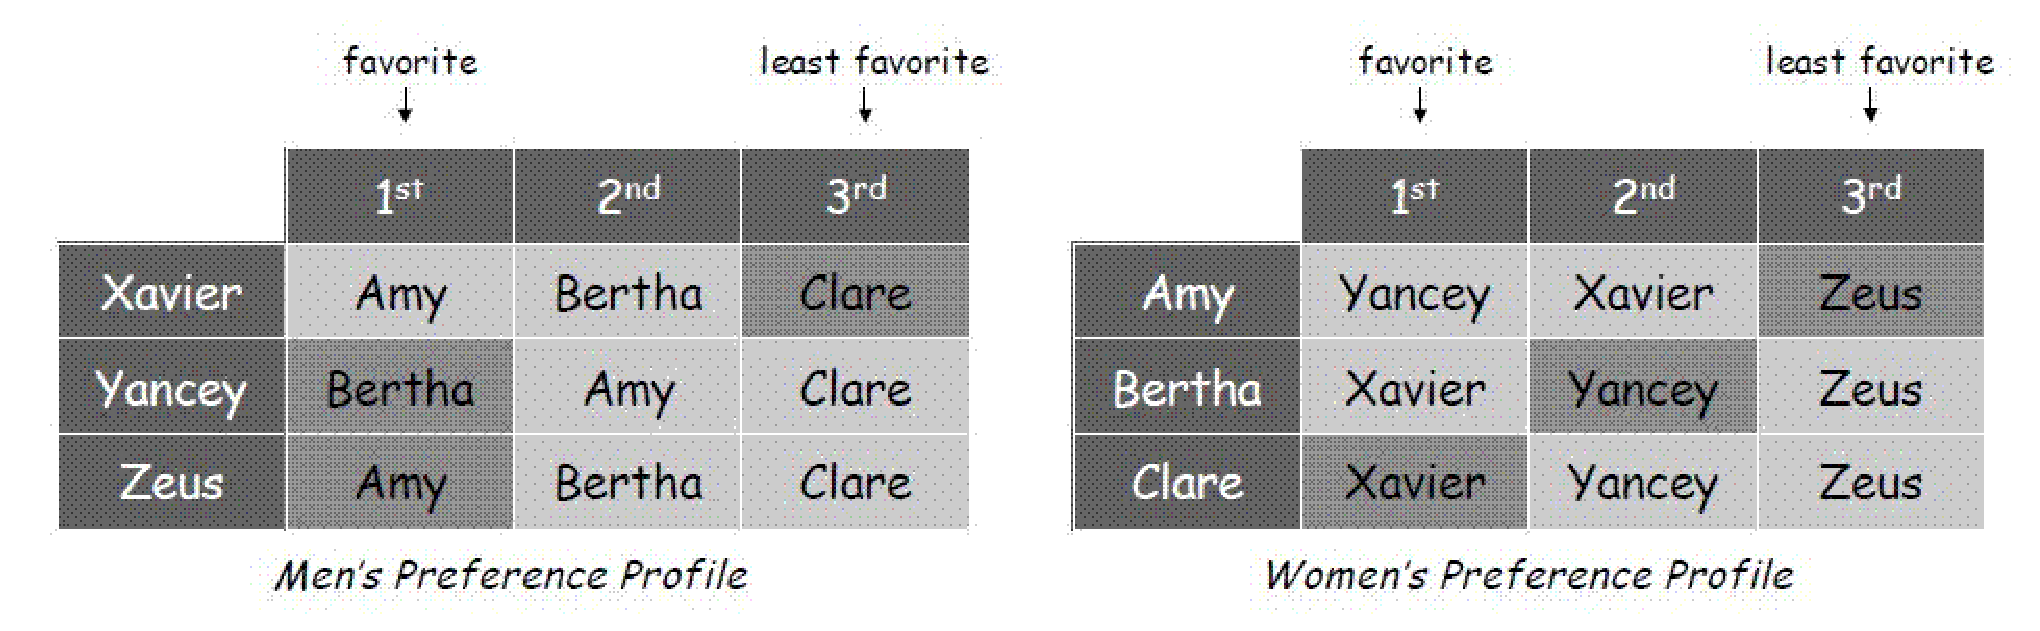
\includegraphics[width=4in] {L1-unstablematchingexampleXYZABC.eps}
\end{figure}

\begin{itemize}
\item The matching $X-A,\ Y-B,\ Z-C$ is stable.
\end{itemize}

\begin{figure}
\begin{tikzpicture}[scale=0.8, auto,swap]
    % Draw a 7,11 network
    % First we draw the vertices
    \foreach \pos/ \name in {{(0,0)/Z},{(0,1.5)/Y},{(0,3)/X}} 
        \node[vertex,fill=blue!20] (\name) at \pos{$\name$};

    \foreach \pos/ \name in {{(3.6,0)/C},{(3.6,1.5)/B},{(3.6,3)/A}} 
        \node[vertex,fill=green] (\name) at \pos {$\name$};
     
    % Connect vertices with edges and draw weights
    \foreach \source/ \dest/\weight in {X/A/{}, Y/B/{}, Z/C/{} }
        \path[undirectededge] (\source) -- node[weight] {$\weight$} (\dest);
%       \draw[dashed, ->] (0,0) arc  (120:60:2);

%\draw[ -latex, blue, line width=5pt ] (5, 1.5) -- (6, 1.5); 

      \end{tikzpicture}

\end{figure}

%\begin{figure}
% \includegraphics[width=1.5in] {L1-stablematchingexample.eps}
%\end{figure}
}

\frame{
  \begin{block}{}
    Question: How to find a stable matching? 
  \end{block}
}

\frame{
	\begin{block}{}
	Trial 1: Improvement strategy
	\end{block}
}

\frame{
  \frametitle{Trial 1: Improvement strategy} 
  \begin{itemize}
    \item Basic idea: starting from a {\bf complete} matching, and try to
{\bf improve} the matching via reducing unstable pairs. If the number of unstable pairs was reduced to 0, then we get a solution. 
    \item {\sc Switching} operation:  making unstable pairs to be stable 


      \item An example of  {\sc Switching} operation:  \\ 

\quad\quad      $m$ prefers $w$ to $w'$; \\
\quad\quad       $m'$ prefers $w$ to $w'$; \\
\quad\quad $w$ prefers $m$ to $m'$; \\
\quad\quad $w'$ prefers $m$ to $m'$; \\
         \end{itemize}
         
         \begin{figure}
\begin{tikzpicture}[scale=1.1, auto,swap]
    % Draw a 7,11 network
    % First we draw the vertices
    \foreach \pos/ \name in {{(0,0)/m'},{(0,1.5)/m}} 
        \node[vertex,fill=blue!20] (\name) at \pos{$\name$};

    \foreach \pos/\name in {{(2,0)/w'}, {(2,1.5)/w}}
        \node[vertex,fill=green] (\name) at \pos {$\name$};
     
    % Connect vertices with edges and draw weights
    \foreach \source/ \dest/\weight in {m/w'/{}, m'/w/{} }
        \path[undirectededge] (\source) -- node[weight] {$\weight$} (\dest);
%       \draw[dashed, ->] (0,0) arc  (120:60:2);

   \foreach \source/ \dest/\weight in {m/w/{}}
        \path[undirectededge, red, dashed] (\source) -- node[weight] {$\weight$} (\dest);

   \node[above] at (1, 2 ) {unstable}; 
   
   
   
   
       \foreach \pos/ \name in {{(4,0)/m'},{(4,1.5)/m}} 
        \node[vertex,fill=blue!20] (\name) at \pos{$\name$};

    \foreach \pos/\name in {{(6,0)/w'}, {(6,1.5)/w}}
        \node[vertex,fill=green] (\name) at \pos {$\name$};
     
    % Connect vertices with edges and draw weights
    \foreach \source/ \dest/\weight in {m/w/{}, m'/w'/{} }
        \path[undirectededge] (\source) -- node[weight] {$\weight$} (\dest);
%       \draw[dashed, ->] (0,0) arc  (120:60:2);

%   \foreach \source/ \dest/\weight in {m/w/{}}
%        \path[undirectededge, red, dashed] (\source) -- node[weight] {$\weight$} (\dest);


   \node[above] at (5, 2 ) {stable}; 
   
   %an arrow
\draw[ -latex, blue, line width=3pt ] (2.7, 0.75) -- (3.3, 0.75); 
   
   
      \end{tikzpicture}

\end{figure}
         
%      \begin{figure}
%        \centering
%        \includegraphics[width=0.8\textwidth]{L1-switching.eps}
%    \end{figure}
%  
}


\frame{
  \frametitle{Trial 1: Improvement strategy } 

\begin{algorithmic}[1]
\STATE Initializing a matching randomly;
\WHILE{ $\exists$ unstable pairs }
\STATE Select an unstable pair $m-w$ arbitrarily ;
\STATE Perform {\sc Switching} operation to resolve the unstable pair  $m-w$;
\ENDWHILE
\end{algorithmic}

}

\frame{
  \frametitle{ Improvement strategy: a success case } 

% \begin{algorithmic}[1]
% \STATE Initializing a randomized matching
% \WHILE{ $\exists$ unstable match }
% \STATE Select an unstable match $m$ arbitrarily 
% \STATE Perform {\sc Switch} operation to make $m$ stable 
% \ENDWHILE
% \end{algorithmic}

\begin{figure}
 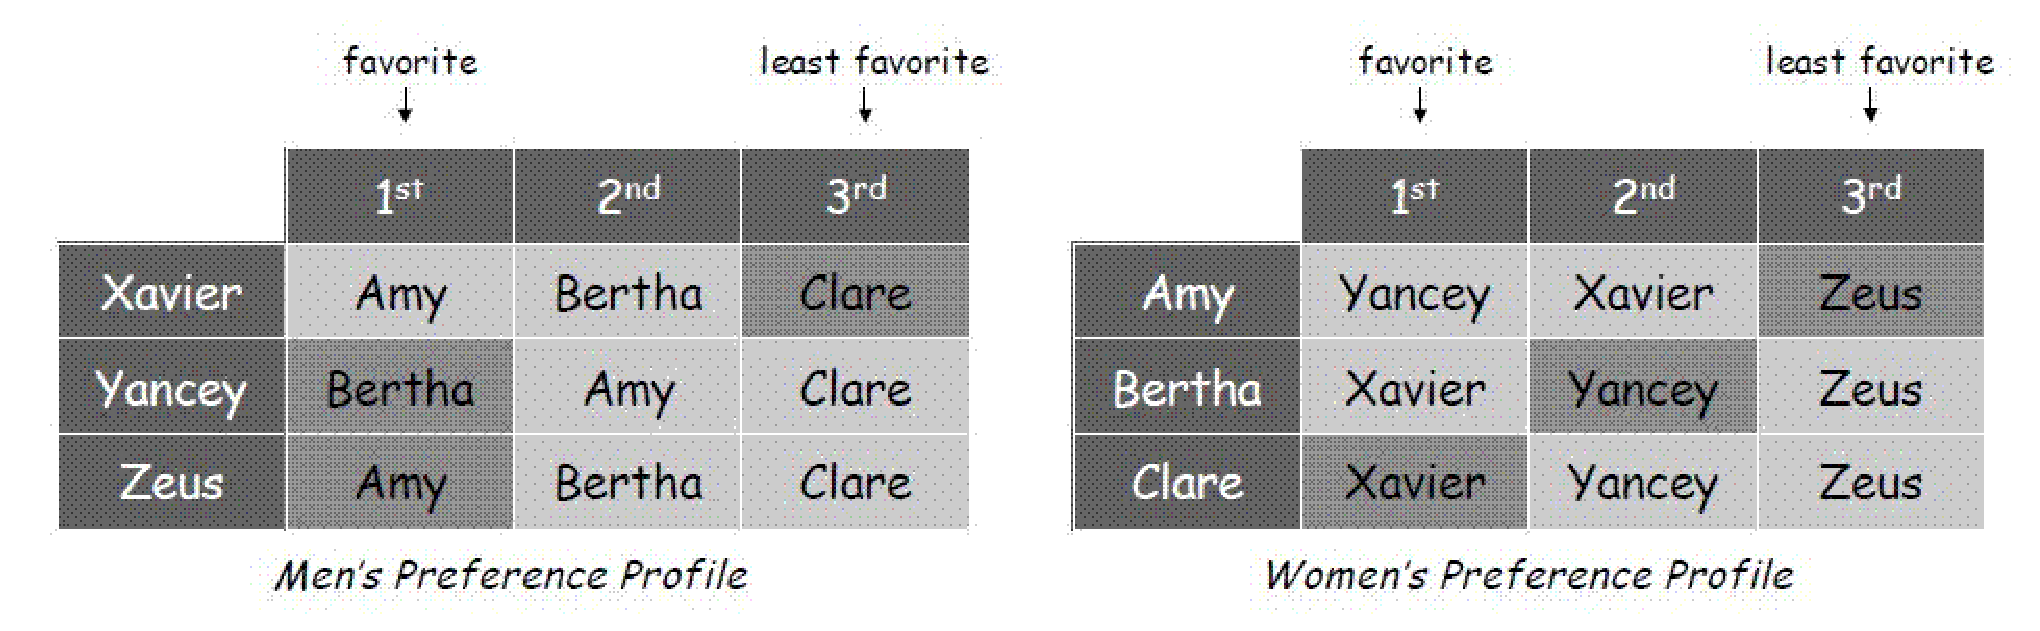
\includegraphics[width=4in] {L1-unstablematchingexampleXYZABC.eps}
\end{figure}
\begin{itemize}
 \item 
Starting from an unstable matching 
\end{itemize}


\begin{figure}
\begin{tikzpicture}[scale=0.8, auto,swap]
    % Draw a 7,11 network
    % First we draw the vertices
    \foreach \pos/ \name in {{(0,0)/Z},{(0,1.5)/Y},{(0,3)/X}} 
        \node[vertex,fill=blue!20] (\name) at \pos{$\name$};

    \foreach \pos/ \name in {{(3.6,0)/C},{(3.6,1.5)/B},{(3.6,3)/A}} 
        \node[vertex,fill=green] (\name) at \pos {$\name$};
     
    % Connect vertices with edges and draw weights
    \foreach \source/ \dest/\weight in {X/C/{}, Y/A/{}, Z/B/{} }
        \path[undirectededge] (\source) -- node[weight] {$\weight$} (\dest);
%       \draw[dashed, ->] (0,0) arc  (120:60:2);

   \foreach \source/ \dest/\weight in {X/B/{}}
        \path[undirectededge, red, dashed] (\source) -- node[weight] {$\weight$} (\dest);
        
%\draw[ -latex, blue, line width=5pt ] (5, 1.5) -- (6, 1.5); 

      \end{tikzpicture}

\end{figure}


%\begin{figure}
% \includegraphics[width=1.5in] {L1-switchingstep0.eps}
%\end{figure}
}

\frame{
  \frametitle{ Improvement strategy: a success case } 

% \begin{algorithmic}[1]
% \STATE Initializing a randomized matching
% \WHILE{ $\exists$ unstable match }
% \STATE Select an unstable match $m$ arbitrarily 
% \STATE Perform {\sc Switch} operation to make $m$ stable 
% \ENDWHILE
% \end{algorithmic}

\begin{figure}
 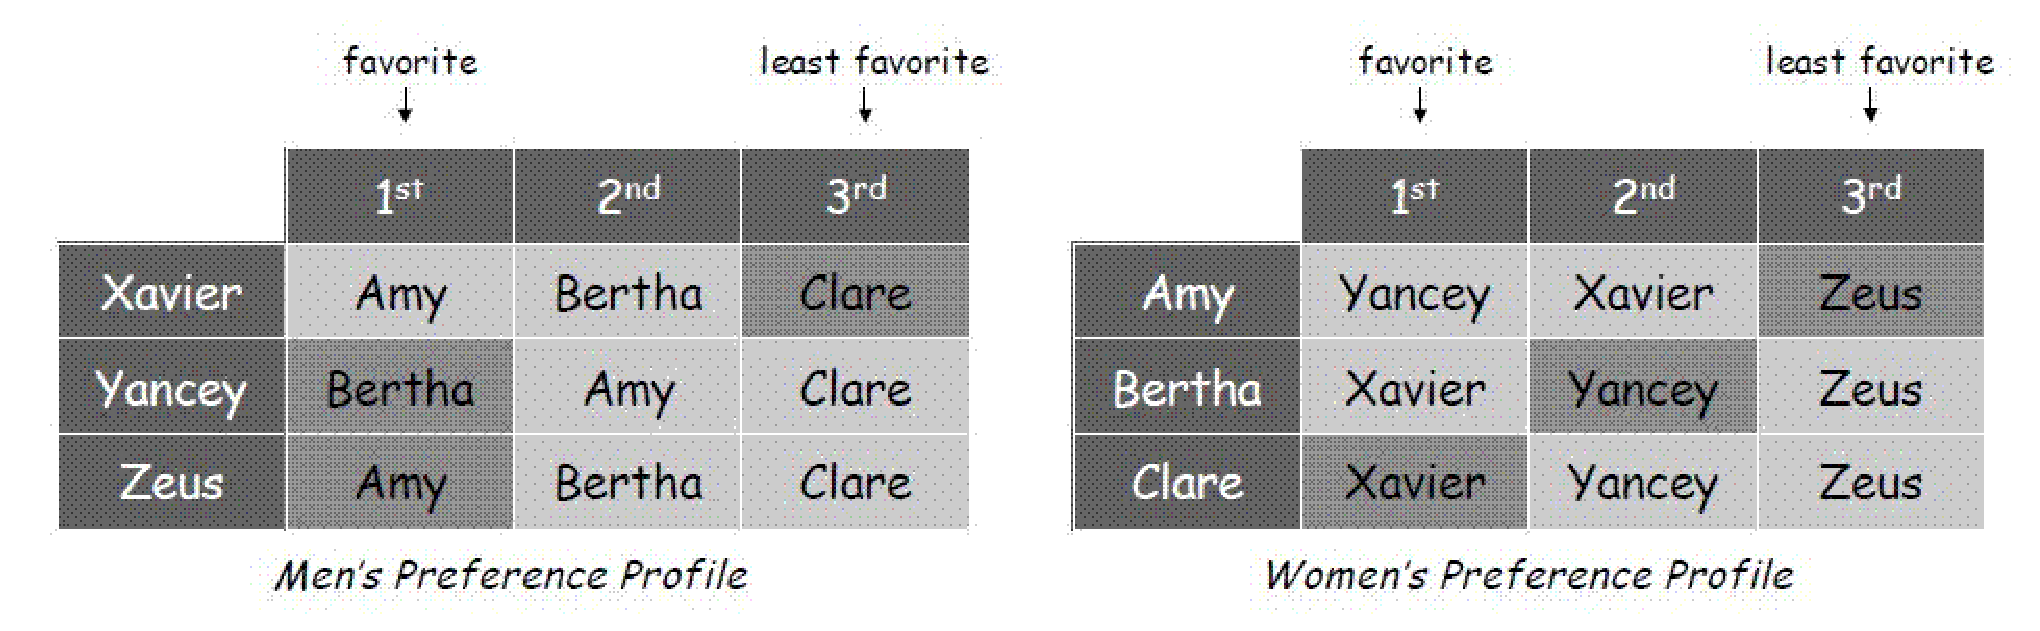
\includegraphics[width=4in] {L1-unstablematchingexampleXYZABC.eps}
\end{figure}
\begin{itemize}
 \item 
After one step of switching, we get a  stable matching. 
\end{itemize}

\begin{figure}
\begin{tikzpicture}[scale=0.8, auto,swap]
    % Draw a 7,11 network
    % First we draw the vertices
    \foreach \pos/ \name in {{(0,0)/Z},{(0,1.5)/Y},{(0,3)/X}} 
        \node[vertex,fill=blue!20] (\name) at \pos{$\name$};

    \foreach \pos/ \name in {{(3.6,0)/C},{(3.6,1.5)/B},{(3.6,3)/A}} 
        \node[vertex,fill=green] (\name) at \pos {$\name$};
     
    % Connect vertices with edges and draw weights
    \foreach \source/ \dest/\weight in {X/C/{}, Y/A/{}, Z/B/{} }
        \path[undirectededge] (\source) -- node[weight] {$\weight$} (\dest);
%       \draw[dashed, ->] (0,0) arc  (120:60:2);

   \foreach \source/ \dest/\weight in {X/B/{}}
        \path[undirectededge, red, dashed] (\source) -- node[weight] {$\weight$} (\dest);
        
\draw[ -latex, blue, line width=3pt ] (4.5, 1.5) -- (5.2, 1.5); 

    \foreach \pos/ \name in {{(6,0)/Z},{(6,1.5)/Y},{(6,3)/X}} 
        \node[vertex,fill=blue!20] (\name) at \pos{$\name$};

    \foreach \pos/ \name in {{(9.6,0)/C},{(9.6,1.5)/B},{(9.6,3)/A}} 
        \node[vertex,fill=green] (\name) at \pos {$\name$};
     
    % Connect vertices with edges and draw weights
    \foreach \source/ \dest/\weight in {X/B/{}, Y/A/{}, Z/C/{} }
        \path[undirectededge] (\source) -- node[weight] {$\weight$} (\dest);
%       \draw[dashed, ->] (0,0) arc  (120:60:2);

%   \foreach \source/ \dest/\weight in {X/B/{}}
%        \path[undirectededge, red, dashed] (\source) -- node[weight] {$\weight$} (\dest);
        
%\draw[ -latex, blue, line width=5pt ] (5, 1.5) -- (6, 1.5); 



      \end{tikzpicture}

\end{figure}

%\begin{figure}
% \includegraphics[width=3.5in] {L1-switchingstep1.eps}
%\end{figure}
}



\frame{
  \frametitle{ Improvement strategy: a failure case } 

  \begin{figure}
 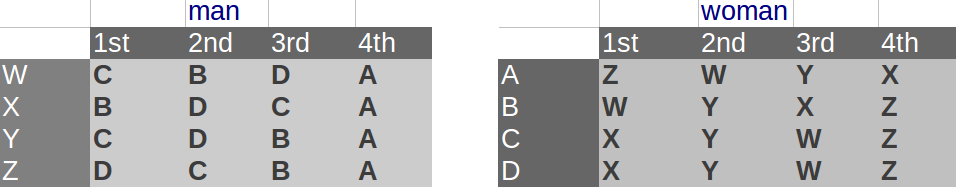
\includegraphics[width=4in] {L1-switchingfailurecase.eps}
\end{figure}
\begin{itemize}
 \item 
Starting from an unstable matching 
\end{itemize}

\begin{figure}
\begin{tikzpicture}[scale=0.8, auto,swap]
    % Draw a 7,11 network
    % First we draw the vertices
    \foreach \pos/ \name in {{(0,0)/Z},{(0,1)/Y},{(0,2)/X}, {(0,3)/W}} 
        \node[vertex,fill=blue!20] (\name) at \pos{$\name$};

    \foreach \pos/ \name in {{(3.6,0)/D},{(3.6,1)/C},{(3.6,2)/B},{(3.6,3)/A}} 
        \node[vertex,fill=green] (\name) at \pos {$\name$};
     
    % Connect vertices with edges and draw weights
    \foreach \source/ \dest/\weight in {W/C/{}, X/D/{}, Y/A/{}, Z/B/{} }
        \path[undirectededge] (\source) -- node[weight] {$\weight$} (\dest);
%       \draw[dashed, ->] (0,0) arc  (120:60:2);

   \foreach \source/ \dest/\weight in {X/B/{}}
        \path[undirectededge, red, dashed] (\source) -- node[weight] {$\weight$} (\dest);
        
%\draw[ -latex, blue, line width=5pt ] (5, 1.5) -- (6, 1.5); 

      \end{tikzpicture}

\end{figure}

%\begin{figure}
% \includegraphics[width=1.5in] {L1-switchingfailurestep0.eps}
%\end{figure}
}


\frame{
  \frametitle{ A failure case: Step 1 } 

  \begin{figure}
 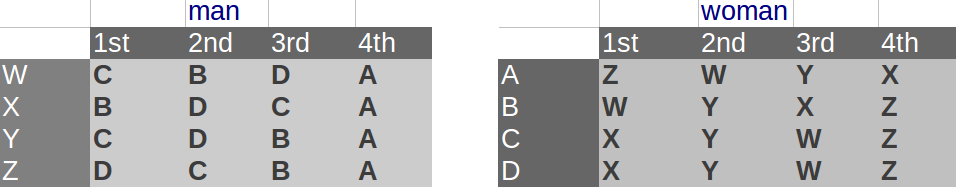
\includegraphics[width=4in] {L1-switchingfailurecase.eps}
\end{figure}


\begin{figure}
\begin{tikzpicture}[scale=0.8, auto,swap]
    % Draw a 7,11 network
    % First we draw the vertices
    \foreach \pos/ \name in {{(0,0)/Z},{(0,1)/Y},{(0,2)/X}, {(0,3)/W}} 
        \node[vertex,fill=blue!20] (\name) at \pos{$\name$};

    \foreach \pos/ \name in {{(3.6,0)/D},{(3.6,1)/C},{(3.6,2)/B},{(3.6,3)/A}} 
        \node[vertex,fill=green] (\name) at \pos {$\name$};
     
    % Connect vertices with edges and draw weights
    \foreach \source/ \dest/\weight in {W/C/{}, X/D/{}, Y/A/{}, Z/B/{} }
        \path[undirectededge] (\source) -- node[weight] {$\weight$} (\dest);
%       \draw[dashed, ->] (0,0) arc  (120:60:2);

   \foreach \source/ \dest/\weight in {X/B/{}}
        \path[undirectededge, red, dashed] (\source) -- node[weight] {$\weight$} (\dest);
        
\draw[ -latex, blue, line width=3pt ] (4.2, 1.5) -- (4.8, 1.5); 

    % Draw a 7,11 network
    % First we draw the vertices
    \foreach \pos/ \name in {{(5.4,0)/Z},{(5.4,1)/Y},{(5.4,2)/X}, {(5.4,3)/W}} 
        \node[vertex,fill=blue!20] (\name) at \pos{$\name$};

    \foreach \pos/ \name in {{(9,0)/D},{(9,1)/C},{(9,2)/B},{(9,3)/A}} 
        \node[vertex,fill=green] (\name) at \pos {$\name$};
     
    % Connect vertices with edges and draw weights
    \foreach \source/ \dest/\weight in {W/C/{}, X/B/{}, Y/A/{}, Z/D/{} }
        \path[undirectededge] (\source) -- node[weight] {$\weight$} (\dest);



      \end{tikzpicture}

\end{figure}


%\begin{figure}
% \includegraphics[width=3.8in] {L1-switchingfailurestep3.eps}
%\end{figure}
}

\frame{
  \frametitle{ A failure case: Step 2 } 

  \begin{figure}
 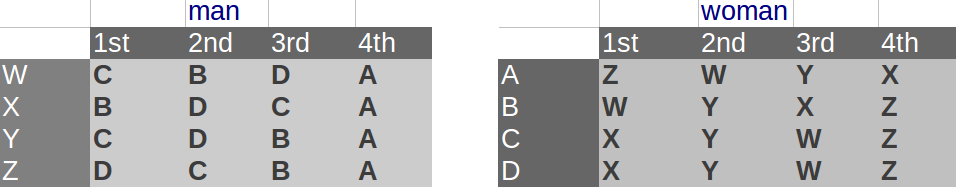
\includegraphics[width=4in] {L1-switchingfailurecase.eps}
\end{figure}

\begin{figure}
\begin{tikzpicture}[scale=0.8, auto,swap]
    % Draw a 7,11 network
    % First we draw the vertices
    \foreach \pos/ \name in {{(0,0)/Z},{(0,1)/Y},{(0,2)/X}, {(0,3)/W}} 
        \node[vertex,fill=blue!20] (\name) at \pos{$\name$};

    \foreach \pos/ \name in {{(3.6,0)/D},{(3.6,1)/C},{(3.6,2)/B},{(3.6,3)/A}} 
        \node[vertex,fill=green] (\name) at \pos {$\name$};
     
    % Connect vertices with edges and draw weights
    \foreach \source/ \dest/\weight in {W/C/{}, X/B/{}, Y/A/{}, Z/D/{} }
        \path[undirectededge] (\source) -- node[weight] {$\weight$} (\dest);
%       \draw[dashed, ->] (0,0) arc  (120:60:2);

   \foreach \source/ \dest/\weight in {Y/B/{}}
        \path[undirectededge, red, dashed] (\source) -- node[weight] {$\weight$} (\dest);
        
\draw[ -latex, blue, line width=3pt ] (4.2, 1.5) -- (4.8, 1.5); 

    % Draw a 7,11 network
    % First we draw the vertices
    \foreach \pos/ \name in {{(5.4,0)/Z},{(5.4,1)/Y},{(5.4,2)/X}, {(5.4,3)/W}} 
        \node[vertex,fill=blue!20] (\name) at \pos{$\name$};

    \foreach \pos/ \name in {{(9,0)/D},{(9,1)/C},{(9,2)/B},{(9,3)/A}} 
        \node[vertex,fill=green] (\name) at \pos {$\name$};
     
    % Connect vertices with edges and draw weights
    \foreach \source/ \dest/\weight in {W/C/{}, X/A/{}, Y/B/{}, Z/D/{} }
        \path[undirectededge] (\source) -- node[weight] {$\weight$} (\dest);



      \end{tikzpicture}

\end{figure}


%\begin{figure}
% \includegraphics[width=3.8in] {L1-switchingfailurestep4.eps}
%\end{figure}
}

\frame{
  \frametitle{ A failure case: Step 3 } 

  \begin{figure}
 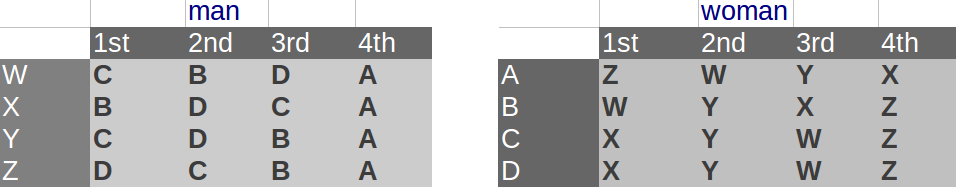
\includegraphics[width=4in] {L1-switchingfailurecase.eps}
\end{figure}

\begin{figure}
\begin{tikzpicture}[scale=0.8, auto,swap]
    % Draw a 7,11 network
    % First we draw the vertices
    \foreach \pos/ \name in {{(0,0)/Z},{(0,1)/Y},{(0,2)/X}, {(0,3)/W}} 
        \node[vertex,fill=blue!20] (\name) at \pos{$\name$};

    \foreach \pos/ \name in {{(3.6,0)/D},{(3.6,1)/C},{(3.6,2)/B},{(3.6,3)/A}} 
        \node[vertex,fill=green] (\name) at \pos {$\name$};
     
    % Connect vertices with edges and draw weights
    \foreach \source/ \dest/\weight in {W/C/{}, X/A/{}, Y/B/{}, Z/D/{} }
        \path[undirectededge] (\source) -- node[weight] {$\weight$} (\dest);
%       \draw[dashed, ->] (0,0) arc  (120:60:2);

   \foreach \source/ \dest/\weight in {X/C/{}}
        \path[undirectededge, red, dashed] (\source) -- node[weight] {$\weight$} (\dest);
        
\draw[ -latex, blue, line width=3pt ] (4.2, 1.5) -- (4.8, 1.5); 

    % Draw a 7,11 network
    % First we draw the vertices
    \foreach \pos/ \name in {{(5.4,0)/Z},{(5.4,1)/Y},{(5.4,2)/X}, {(5.4,3)/W}} 
        \node[vertex,fill=blue!20] (\name) at \pos{$\name$};

    \foreach \pos/ \name in {{(9,0)/D},{(9,1)/C},{(9,2)/B},{(9,3)/A}} 
        \node[vertex,fill=green] (\name) at \pos {$\name$};
     
    % Connect vertices with edges and draw weights
    \foreach \source/ \dest/\weight in {W/A/{}, X/C/{}, Y/B/{}, Z/D/{} }
        \path[undirectededge] (\source) -- node[weight] {$\weight$} (\dest);



      \end{tikzpicture}

\end{figure}

%
%\begin{figure}
% \includegraphics[width=3.8in] {L1-switchingfailurestep5.eps}
%\end{figure}
}

\frame{
  \frametitle{ A failure case: Step 4 } 

  \begin{figure}
 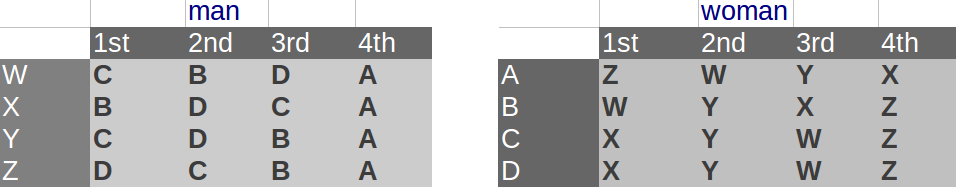
\includegraphics[width=4in] {L1-switchingfailurecase.eps}
\end{figure}

\begin{figure}
\begin{tikzpicture}[scale=0.8, auto,swap]
    % Draw a 7,11 network
    % First we draw the vertices
    \foreach \pos/ \name in {{(0,0)/Z},{(0,1)/Y},{(0,2)/X}, {(0,3)/W}} 
        \node[vertex,fill=blue!20] (\name) at \pos{$\name$};

    \foreach \pos/ \name in {{(3.6,0)/D},{(3.6,1)/C},{(3.6,2)/B},{(3.6,3)/A}} 
        \node[vertex,fill=green] (\name) at \pos {$\name$};
     
    % Connect vertices with edges and draw weights
    \foreach \source/ \dest/\weight in {W/A/{}, X/C/{}, Y/B/{}, Z/D/{} }
        \path[undirectededge] (\source) -- node[weight] {$\weight$} (\dest);
%       \draw[dashed, ->] (0,0) arc  (120:60:2);

   \foreach \source/ \dest/\weight in {W/B/{}}
        \path[undirectededge, red, dashed] (\source) -- node[weight] {$\weight$} (\dest);
        
\draw[ -latex, blue, line width=3pt ] (4.2, 1.5) -- (4.8, 1.5); 

    % Draw a 7,11 network
    % First we draw the vertices
    \foreach \pos/ \name in {{(5.4,0)/Z},{(5.4,1)/Y},{(5.4,2)/X}, {(5.4,3)/W}} 
        \node[vertex,fill=blue!20] (\name) at \pos{$\name$};

    \foreach \pos/ \name in {{(9,0)/D},{(9,1)/C},{(9,2)/B},{(9,3)/A}} 
        \node[vertex,fill=green] (\name) at \pos {$\name$};
     
    % Connect vertices with edges and draw weights
    \foreach \source/ \dest/\weight in {W/B/{}, X/C/{}, Y/A/{}, Z/D/{} }
        \path[undirectededge] (\source) -- node[weight] {$\weight$} (\dest);



      \end{tikzpicture}

\end{figure}


%\begin{figure}
% \includegraphics[width=3.8in] {L1-switchingfailurestep6.eps}
%\end{figure}
}

\frame{
  \frametitle{ A failure case: Step 5 } 

  \begin{figure}
 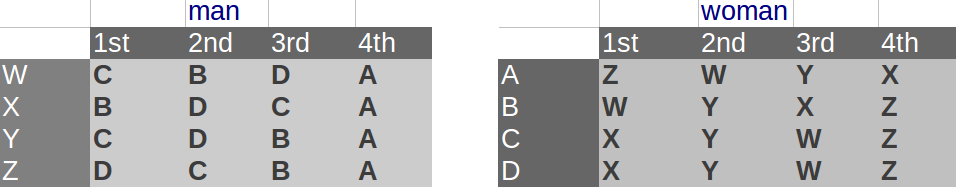
\includegraphics[width=4in] {L1-switchingfailurecase.eps}
\end{figure}

\begin{figure}
\begin{tikzpicture}[scale=0.8, auto,swap]
    % Draw a 7,11 network
    % First we draw the vertices
    \foreach \pos/ \name in {{(0,0)/Z},{(0,1)/Y},{(0,2)/X}, {(0,3)/W}} 
        \node[vertex,fill=blue!20] (\name) at \pos{$\name$};

    \foreach \pos/ \name in {{(3.6,0)/D},{(3.6,1)/C},{(3.6,2)/B},{(3.6,3)/A}} 
        \node[vertex,fill=green] (\name) at \pos {$\name$};
     
    % Connect vertices with edges and draw weights
    \foreach \source/ \dest/\weight in {W/B/{}, X/C/{}, Y/A/{}, Z/D/{} }
        \path[undirectededge] (\source) -- node[weight] {$\weight$} (\dest);
%       \draw[dashed, ->] (0,0) arc  (120:60:2);

   \foreach \source/ \dest/\weight in {X/D/{}}
        \path[undirectededge, red, dashed] (\source) -- node[weight] {$\weight$} (\dest);
        
\draw[ -latex, blue, line width=3pt ] (4.2, 1.5) -- (4.8, 1.5); 

    % Draw a 7,11 network
    % First we draw the vertices
    \foreach \pos/ \name in {{(5.4,0)/Z},{(5.4,1)/Y},{(5.4,2)/X}, {(5.4,3)/W}} 
        \node[vertex,fill=blue!20] (\name) at \pos{$\name$};

    \foreach \pos/ \name in {{(9,0)/D},{(9,1)/C},{(9,2)/B},{(9,3)/A}} 
        \node[vertex,fill=green] (\name) at \pos {$\name$};
     
    % Connect vertices with edges and draw weights
    \foreach \source/ \dest/\weight in {W/B/{}, X/D/{}, Y/A/{}, Z/C/{} }
        \path[undirectededge] (\source) -- node[weight] {$\weight$} (\dest);



      \end{tikzpicture}

\end{figure}

%\begin{figure}
% \includegraphics[width=3.8in] {L1-switchingfailurestep1.eps}
%\end{figure}
}

\frame{
  \frametitle{ A failure case: Step 6 } 

  \begin{figure}
 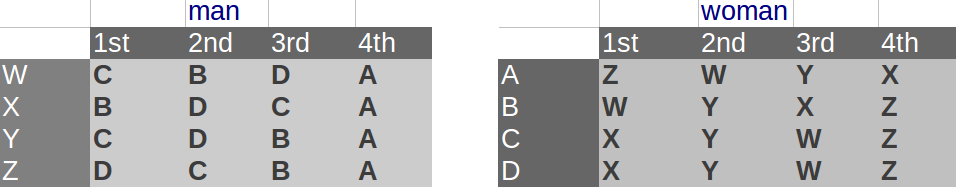
\includegraphics[width=4in] {L1-switchingfailurecase.eps}
\end{figure}

\begin{figure}
\begin{tikzpicture}[scale=0.8, auto,swap]
    % Draw a 7,11 network
    % First we draw the vertices
    \foreach \pos/ \name in {{(0,0)/Z},{(0,1)/Y},{(0,2)/X}, {(0,3)/W}} 
        \node[vertex,fill=blue!20] (\name) at \pos{$\name$};

    \foreach \pos/ \name in {{(3.6,0)/D},{(3.6,1)/C},{(3.6,2)/B},{(3.6,3)/A}} 
        \node[vertex,fill=green] (\name) at \pos {$\name$};
     
    % Connect vertices with edges and draw weights
    \foreach \source/ \dest/\weight in {W/B/{}, X/D/{}, Y/A/{}, Z/C/{} }
        \path[undirectededge] (\source) -- node[weight] {$\weight$} (\dest);
%       \draw[dashed, ->] (0,0) arc  (120:60:2);

   \foreach \source/ \dest/\weight in {W/C/{}}
        \path[undirectededge, red, dashed] (\source) -- node[weight] {$\weight$} (\dest);
        
\draw[ -latex, blue, line width=3pt ] (4.2, 1.5) -- (4.8, 1.5); 

    % Draw a 7,11 network
    % First we draw the vertices
    \foreach \pos/ \name in {{(5.4,0)/Z},{(5.4,1)/Y},{(5.4,2)/X}, {(5.4,3)/W}} 
        \node[vertex,fill=blue!20] (\name) at \pos{$\name$};

    \foreach \pos/ \name in {{(9,0)/D},{(9,1)/C},{(9,2)/B},{(9,3)/A}} 
        \node[vertex,fill=green] (\name) at \pos {$\name$};
     
    % Connect vertices with edges and draw weights
    \foreach \source/ \dest/\weight in {W/C/{}, X/D/{}, Y/A/{}, Z/B/{} }
        \path[undirectededge] (\source) -- node[weight] {$\weight$} (\dest);



      \end{tikzpicture}

\end{figure}

%
%\begin{figure}
% \includegraphics[width=3.8in] {L1-switchingfailurestep2.eps}
%\end{figure}
\begin{itemize}
\item 
Failed! Return to the initial matching. 
\end{itemize}
}

% \frame{
%  \frametilte{Trial 2: Increment strategy} 
%  
%  Key observations: 
%  \begin{itemize}
%  \item Solution: match \\
%  \item Space size: $O(n!)$\\
%  \item Brute-force: enumerating all possible matches. \\
%  \end{itemize}
% \begin{figure}
%  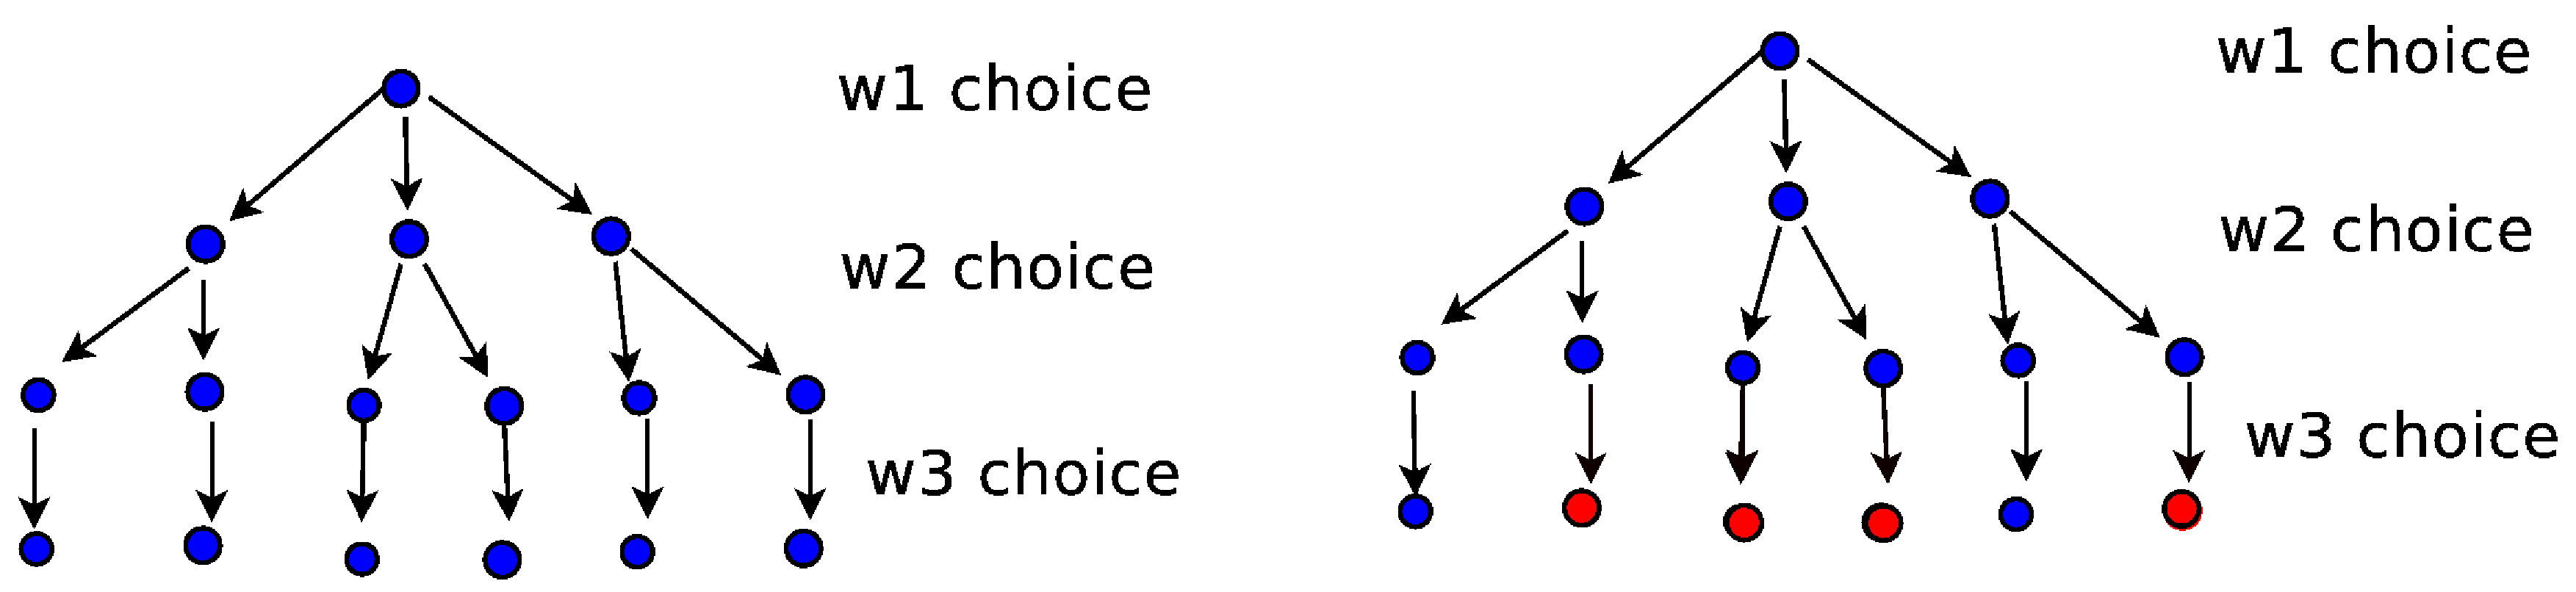
\includegraphics[width=4in] {L1-stablematchsearchspace.eps}
% \end{figure}
% }
\frame{
	\begin{block}{}
	Trial 2: Increment strategy
	\end{block}
}

\frame{
 \frametitle{Trial 2: Increment strategy}
 \begin{itemize}
 \item Key observation: the solution is a {\bf compelte} matching. 
 \item Basic idea: Growing up from {\bf partial} matching to
{\bf complete} matching, and ensure no unstable pairs during the
increment process. \\
 \item Implementation:  a ``propose-engage'' process. Man: propose, woman:
accept or reject.
 \end{itemize}
 
 \begin{figure}
\begin{tikzpicture}[scale=1, auto,swap]
   
   
       \foreach \pos/ \name in {{(0,0)/m''},{(0,1)/m'},{(0,2)/m}} 
        \node[vertex,fill=blue!20] (\name) at \pos{$\name$};

    \foreach \pos/ \name in {{(2.4,0)/w''},{(2.4,1)/w'},{(2.4,2)/w}} 
        \node[vertex,fill=green] (\name) at \pos {$\name$};
     
    % Connect vertices with edges and draw weights
    \foreach \source/ \dest/\weight in {m/w'/{}, m'/w/{}, m''/w''/{} }
        \path[undirectededge] (\source) -- node[weight] {$\weight$} (\dest);

%   \foreach \source/ \dest/\weight in {W/C/{}}
%        \path[undirectededge, red, dashed] (\source) -- node[weight] {$\weight$} (\dest);
%        
%\draw[ -latex, blue, line width=3pt ] (4.2, 1.5) -- (4.8, 1.5); 

      \foreach \pos/ \name in {{(4.4,0)/m''},{(4.4,1)/m'},{(4.4,2)/m}} 
        \node[vertex,fill=blue!20] (\name) at \pos{$\name$};

    \foreach \pos/ \name in {{(6.8,0)/w''},{(6.8,1)/w'},{(6.8,2)/w}} 
        \node[vertex,fill=green] (\name) at \pos {$\name$};
     
    % Connect vertices with edges and draw weights
    \foreach \source/ \dest/\weight in {m/w'/{},  m''/w''/{} }
        \path[undirectededge] (\source) -- node[weight] {$\weight$} (\dest);


 \node[below] at (1.2, -0.5) {complete  solution}; 
 \node[below] at (5.5, -0.5) {partial  solution}; 
 
      \end{tikzpicture}

\end{figure}


%\begin{figure}
% \includegraphics[width=3.4in] {L1-stablematchgloballocal.eps}
%\end{figure}
}

\frame
{
\frametitle{Stable Matching -- Gale\_Shapley algorithm }
% An intuitive method that guarantees to find a stable matching:\\
% \begin{algorithm}[1]
% \caption{Calculate $y = x^n$}
 %\label{alg1}
\begin{footnotesize}
\begin{algorithmic}[1]
\FOR{$m=1$ to $M$} 
\STATE $partner[m] \ = \ NULL $ \ENDFOR
\FOR{$w=1$ to $W$} 
\STATE $partner[w] \ = \ NULL $ \ENDFOR
\WHILE{ TRUE }
\IF{ there is no man $m$ such that $partner[m]=NULL$ }
\STATE return; 
\ENDIF
\STATE select such a man $m$ \textcolor{red}{arbitrarily};
\STATE $w = $ the first woman on $m'$s list to whom $m$ have not yet proposed;
\IF{$partner[w] == NULL $}
\STATE $partner[w]=m;  partner[m]=w;$
\ELSIF{$w$ prefers $m$ to $partner[w]$ }
\STATE $partner[ partner[w] ] = NULL; \ partner[w]=m; \ partner[m]=w;$
\ELSE{}
\STATE ; //do nothing means simply rejecting m;
\ENDIF
\ENDWHILE
\end{algorithmic}
\end{footnotesize}

%  \begin{figure}
%   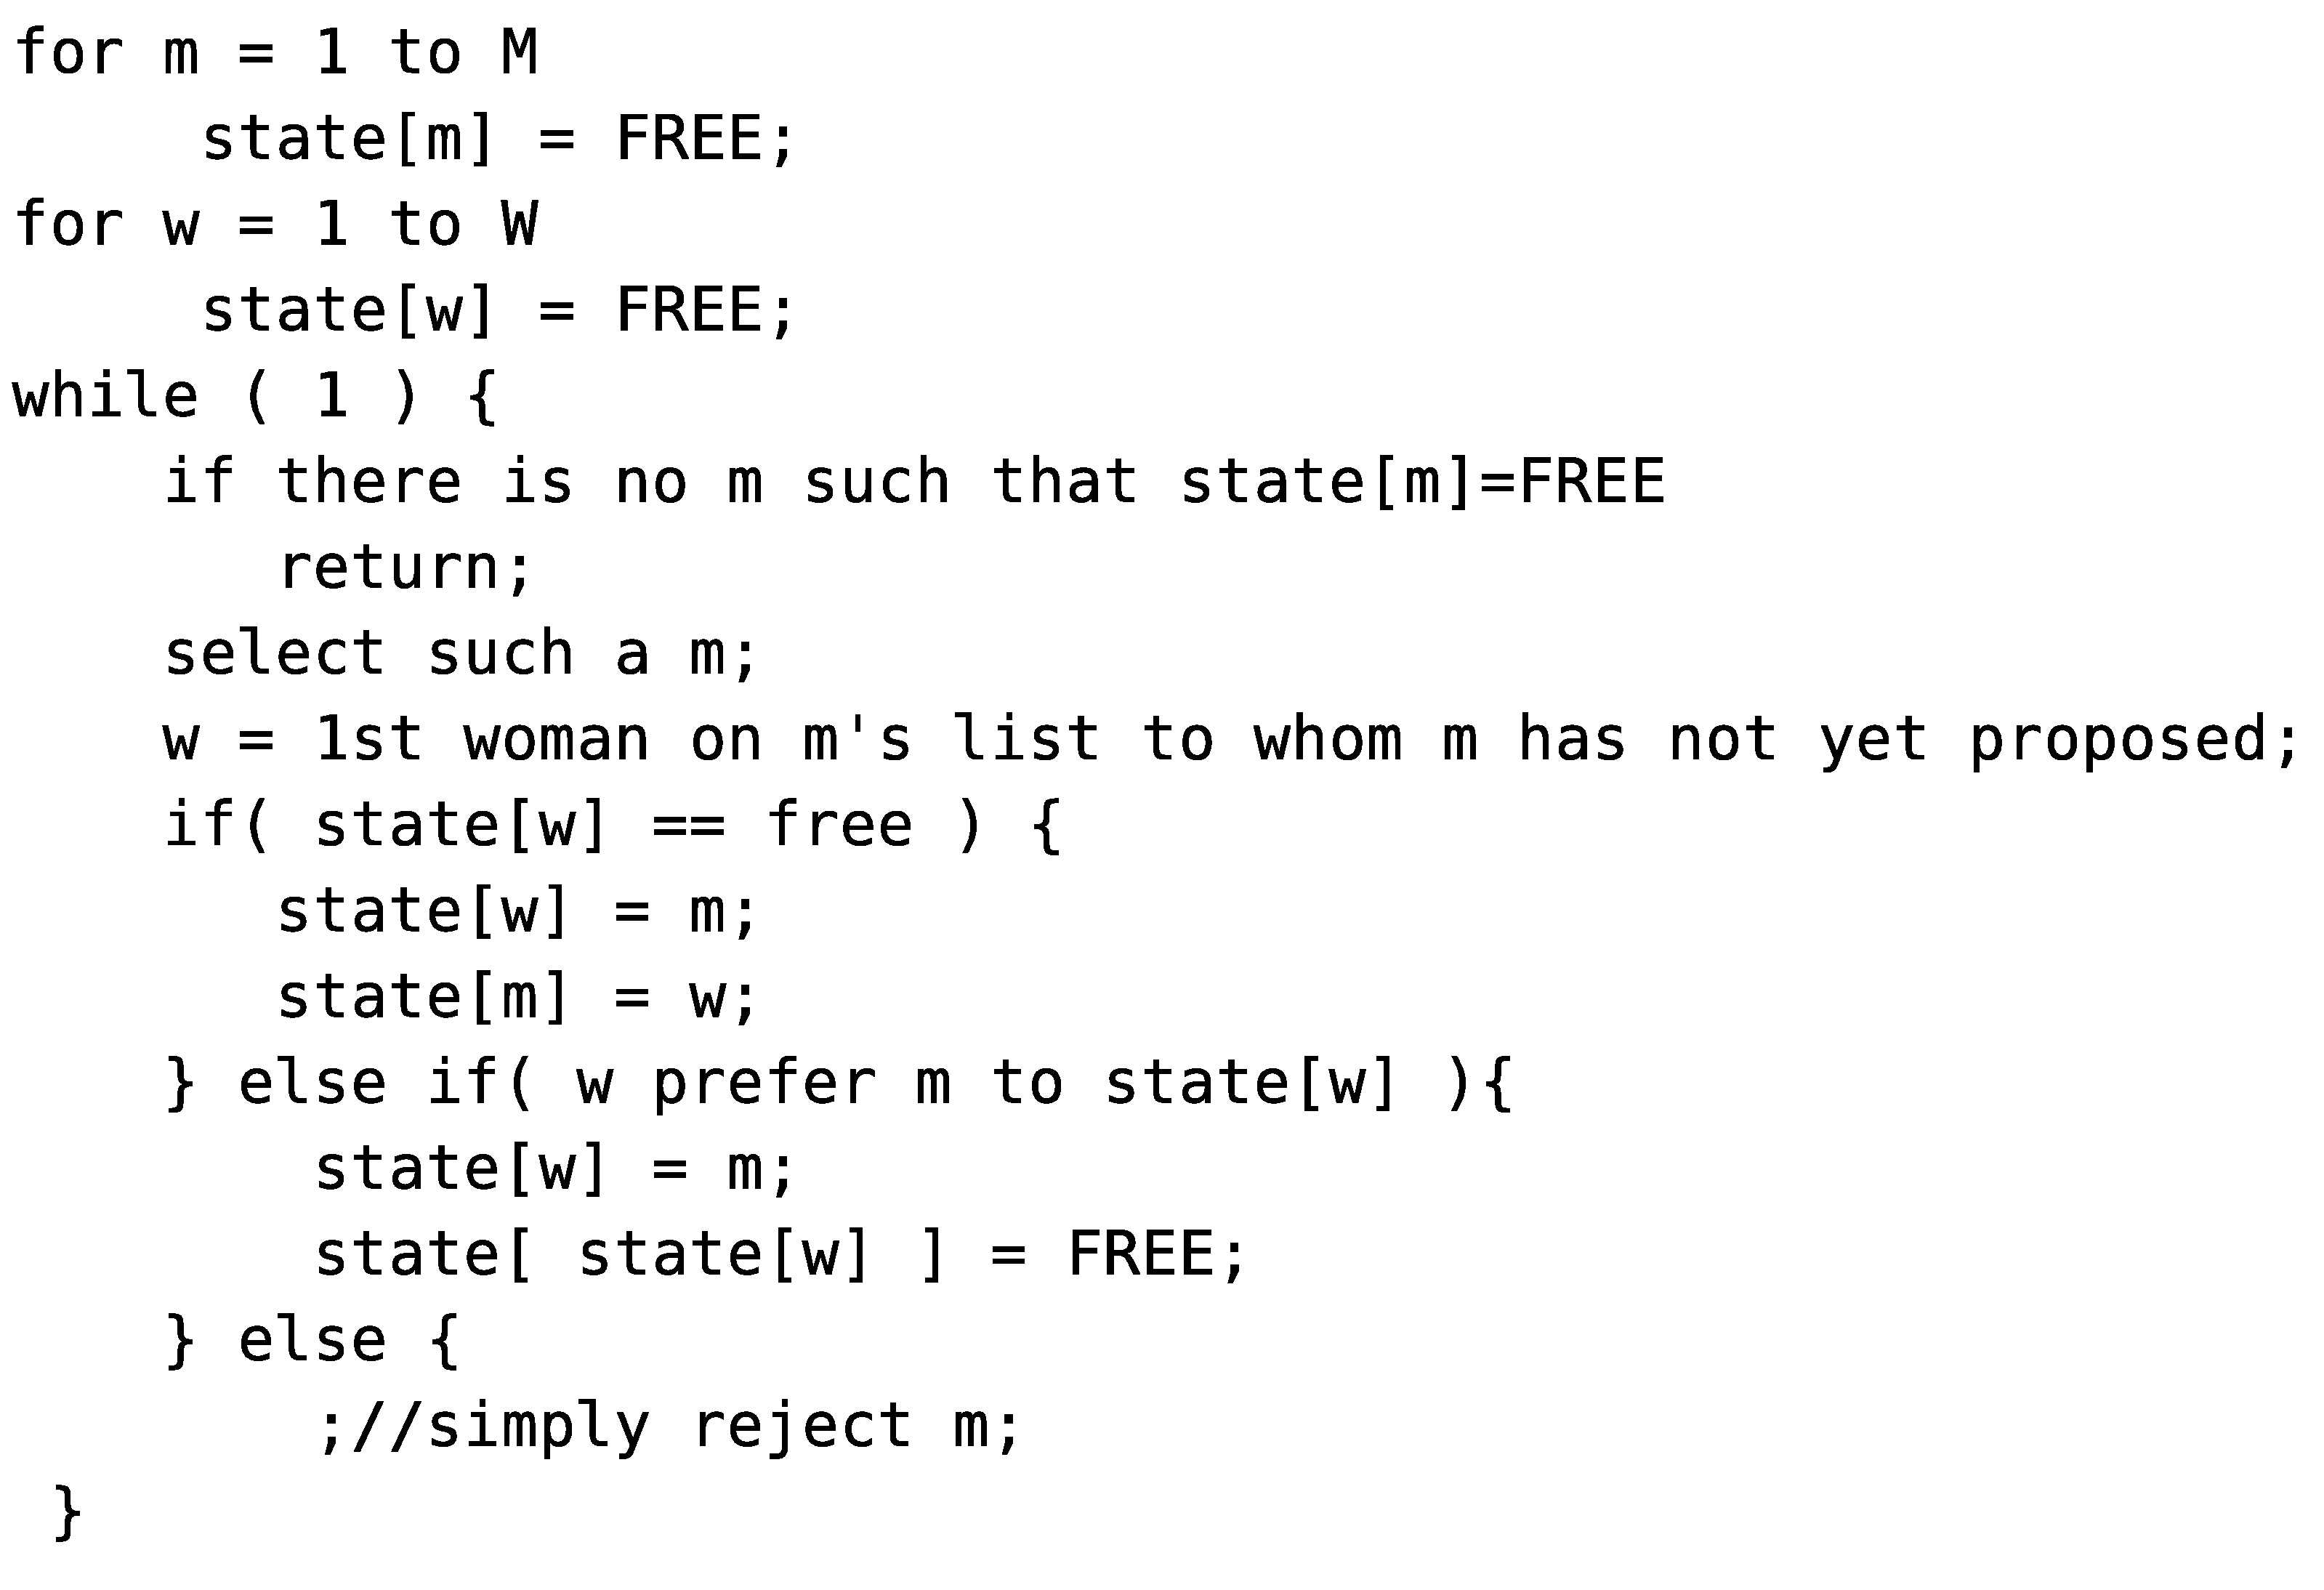
\includegraphics[width=4in] {L1-GS-algo.eps}
%  \end{figure}
(see ppt for a demo)
}

\frame{
	\begin{block}{}
	Correctness proof
	\end{block}
}

\frame{
\frametitle{Key observations of Gale\_Shapley algorithm }
Key observations: \\
\begin{enumerate}
 \item Men propose to women in the decreasing order of preference. 
\item Once a woman is matched, she never becomes unmatched. 
\item When a man proposes, the existing matching might be destroyed. 
\end{enumerate}

}


\frame{
\frametitle{Correctness: perfection}
\begin{Theorem}
 All men and women finally get matched.
\end{Theorem}
\begin{Proof}
 Suppose $m''$ is not matched upon termination; \\
\begin{itemize}
 \item then there is woman, say $w''$, is not matched;
 \item then $w''$ should be never proposed to (by Observation 2);
 \item But $m''$ proposes to everyone. Contradiction.
 \begin{figure}
\begin{tikzpicture}[scale=1.0, auto,swap]
   
   
       \foreach \pos/ \name in {{(0,0)/m''},{(0,1)/m'},{(0,2)/m}} 
        \node[vertex,fill=blue!20] (\name) at \pos{$\name$};

    \foreach \pos/ \name in {{(2.4,0)/w''},{(2.4,1)/w'},{(2.4,2)/w}} 
        \node[vertex,fill=green] (\name) at \pos {$\name$};
     
    % Connect vertices with edges and draw weights
    \foreach \source/ \dest/\weight in {m/w'/{}, m'/w/{} }
        \path[undirectededge] (\source) -- node[weight] {$\weight$} (\dest);

%   \foreach \source/ \dest/\weight in {W/C/{}}
%        \path[undirectededge, red, dashed] (\source) -- node[weight] {$\weight$} (\dest);
%        
%\draw[ -latex, blue, line width=3pt ] (4.2, 1.5) -- (4.8, 1.5); 

      \end{tikzpicture}

\end{figure}

%\begin{figure}
% \includegraphics[width=1.2in] {L1-stablematchperfection.eps}
%\end{figure}
\end{itemize}
\end{Proof}
}


\frame{
\frametitle{Correctness: stability}
\begin{theorem}
 At each step of the while loop, the inter-mediate partial match is a stable match. As a special case, the finally reported match $S^*$ contains no unstable pairs. 
\end{theorem}
\begin{Proof}
  Suppose $m-w'$ is an unstable pair: each prefers the other to the current partner in $S^*$;

\begin{itemize}
 \item Case 1: $m$ never proposed to $w'$  \\
  $\Rightarrow$ $m$ prefers his GS partner $w$ to $w'$ \\
    $\Rightarrow$ $m-w'$ is stable. A contradiction.  \\
    
    \begin{figure}
\begin{tikzpicture}[scale=1., auto,swap]
   
   
       \foreach \pos/ \name in {{(0,1)/m'},{(0,2)/m}} 
        \node[vertex,fill=blue!20] (\name) at \pos{$\name$};

    \foreach \pos/ \name in {{(2.4,1)/w'},{(2.4,2)/w}} 
        \node[vertex,fill=green] (\name) at \pos {$\name$};
     
    % Connect vertices with edges and draw weights
    \foreach \source/ \dest/\weight in {m/w/{}, m'/w'/{} }
        \path[undirectededge] (\source) -- node[weight] {$\weight$} (\dest);

   \foreach \source/ \dest/\weight in {m/w'/{}}
        \path[undirectededge, red, dashed] (\source) -- node[weight] {$\weight$} (\dest);
%        
%\draw[ -latex, blue, line width=3pt ] (4.2, 1.5) -- (4.8, 1.5); 

      \end{tikzpicture}

\end{figure}

%\begin{figure}
% \includegraphics[width=3in] {L1-stablematchcase2.eps}
%\end{figure}

\end{itemize}
\end{Proof}
}


\frame{
\frametitle{Correctness: stability}
\begin{itemize}
 \item Case 2: $m$ has proposed to $w'$ \\
$\Rightarrow$ $m$ should be rejected by $w'$  \\
   $\Rightarrow$ $w'$ prefer her GS partner $m'$ to $m$ \\
  $\Rightarrow$ $m-w'$ is stable. A contradiction.
  
  \begin{figure}
\begin{tikzpicture}[scale=1., auto,swap]
   
   
       \foreach \pos/ \name in {{(0,1)/m'},{(0,2)/m}} 
        \node[vertex,fill=blue!20] (\name) at \pos{$\name$};

    \foreach \pos/ \name in {{(2.4,1)/w'},{(2.4,2)/w}} 
        \node[vertex,fill=green] (\name) at \pos {$\name$};
     
    % Connect vertices with edges and draw weights
    \foreach \source/ \dest/\weight in {m/w/{}, m'/w'/{} }
        \path[undirectededge] (\source) -- node[weight] {$\weight$} (\dest);

   \foreach \source/ \dest/\weight in {m/w'/{}}
        \path[undirectededge, red, dashed] (\source) -- node[weight] {$\weight$} (\dest);
%        
%\draw[ -latex, blue, line width=3pt ] (4.2, 1.5) -- (4.8, 1.5); 

       \foreach \pos/ \name in {{(3.6,1)/m'},{(3.6,2)/m}} 
        \node[vertex,fill=blue!20] (\name) at \pos{$\name$};

    \foreach \pos/ \name in {{(6,1)/w'},{(6,2)/w}} 
        \node[vertex,fill=green] (\name) at \pos {$\name$};
     
    % Connect vertices with edges and draw weights
    \foreach \source/ \dest/\weight in {m/w/{}, m'/w'/{} }
        \path[undirectededge] (\source) -- node[weight] {$\weight$} (\dest);

   \foreach \source/ \dest/\weight in {m/w'/{}}
        \path[edge, blue] (\source) -- node[weight] {$\weight$} (\dest);

 \node[color=red] at (4.8, 1.5) {Reject}; 

      \end{tikzpicture}

\end{figure}


%\begin{figure}
% \includegraphics[width=3in] {L1-stablematchcase1.eps}
%\end{figure}
%

\end{itemize}
}
   
   
   \frame{
	\begin{block}{}
	Algorithm analysis:  time complexity and space complexity
	\end{block}
}



\frame{
\frametitle{Analysis: time-complexity}
\begin{Theorem}
 Gale-Shapley  algorithm ends in $O(n^2)$ steps. 
\end{Theorem}
 \begin{Proof}
\begin{itemize}
 \item 
 Key: find a measure of progress for this $while (1)$ type loop; \\
 \item 
 Measure: the number of tried proposals $\#P$; \\
\end{itemize}
 
 (see an extra slide) 
 
   \end{Proof}
} 

\frame{
\frametitle{Analysis: time-complexity}
 
\begin{itemize}
 \item 
 Each step: $\#P$ increases at least $1$;  \\
 \item 
Upper bound: $\#P \le n^2$ \\
\item
So $T(n) = \#Step \le n^2$; \\
\end{itemize}

\begin{itemize}
 \item 
Try other measures:  \\
\begin{enumerate}
\item 
the number of matches \\
\item 
the number of engaged women \\
\item 
the sum of preference 
\end{enumerate}
\item Note: we will revisit {\sc Stable Matching} problem later.
\end{itemize} 
}

\frame{
\frametitle{Time complexity and space complexity}

\begin{itemize}
	\item Time (space) complexity of an algorithm quantifies the time (space) taken by the algorithm. 
	\item Since the time costed by an algorithm grows with the size of the input, it is traditional to describe running time as a  function of the input size. 
	\begin{itemize}		
		\item \textcolor{blue}{\bf input size}: The best notion of input size depends on the problem being studied. 
			\begin{itemize}
				\item For the {\sc Stable Matching} problem, the \textcolor{blue}{\tt number of items in the input}, i.e. the number of men, is the natural measure. 
				\item For the {\sc Multiplication} problem, the \textcolor{blue}{\tt total number of bits} needed to represent the input number is the best measure. 
			\end{itemize}		  		
	\end{itemize}
\end{itemize}
} 

\frame{
\frametitle{Running time:  we are interested in its growth rate}
\begin{itemize}
	\item Several  simplifications to ease  analysis of  Gale-Shapley  algorithm: 
	\begin{enumerate}
		\item  We simply use the number of primitive operations (rather than the exact seconds used) under the assumption that a primitive operation costs constant time. Thus the running time is $T(n) = a n^2 + b n + c $ for some constants $a, b, c$. 
		\item We consider only the leading term, i.e. $a n^2$, since the lower order terms are relatively insignificant for large $n$. 
		\item We also ignore the leading term's coefficient $a$ since the it is less significant than the growth rate. 
	\end{enumerate} 
	\item Thus, we have $T(n) = a n^2 + b n + c = O(n^2)$.  Here, the letter $O$ denotes \textcolor{blue}{order}.  
\end{itemize}
} 

\frame{
\frametitle{ \textcolor{red}{Big $O$}  notation } 

\begin{itemize}
	\item Recall that big $O$ notation is used to describe the \textcolor{blue}{\tt error term} in Taylor series, say: 
	
	\centering{$e^x = 1 + x + \frac{x^2}{2} + O(x^3)$ as $x\rightarrow 0 $ }
	
\end{itemize}

\begin{figure}
 \includegraphics[width=1.6in,angle=270] {L1-big-O.eps}
 \caption{Example: $f(x) = O(g(x))$ as there exists $c>0$ (e.g. $c=1$) and $x_0 = 5$ such that 
 $f(x) < c g(x)$ whenever $x>x_0$} 
\end{figure}

}

\frame{
\frametitle{ \textcolor{red}{Big $\Omega$} and  \textcolor{red}{Big $\Theta$}  notations } 

\begin{itemize}
\item 
In 1976 D.E. Knuth published a paper  to justify his use of the $\Omega$-symbol to describe a stronger property. Knuth wrote: "For all the applications I have seen so far in computer science, a stronger requirement … is much more appropriate". 

\item He defined

\begin{center} 
$f(x)=\Omega(g(x))\Leftrightarrow g(x)=O(f(x))$
\end{center}

with the comment: "Although I have changed Hardy and Littlewood's definition of $\Omega$, I feel justified in doing so because their definition is by no means in wide use, and because there are other ways to say what they want to say in the comparatively rare cases when their definition applies". 

\item Big $\Theta$ notation is used to describe ``$f(n)$ grows  asymptotically as fast as $g(n)$". 
\begin{center} 
$f(x)=\Theta(g(x))\Leftrightarrow g(x)=O(f(x)) $ and $f(x) = O(g(x))$. 
\end{center}

\end{itemize}
%However, the Hardy–Littlewood definition had been used for at least 25 years.[13]
}




\frame{
\begin{block}{}
Extension: a bit strange observation
\end{block}
}

\frame{
\frametitle{A bit strange observation}
\begin{theorem}
 Any execution of Gale\_Shapley algorithm yields the same matching $S^*$.
\end{theorem}

Note: 
\begin{itemize}
	\item The theorem is non-trial since in line 11, an unmatched man $m$ is selected \textcolor{red}{arbitrarily.} 
\end{itemize} 

Notations: 	
\begin{itemize}
 \item 
\textcolor{blue}{\bf Valid partner:} $w$ is a valid partner of $m$ if the pair $m-w$ exists in a stable match; \\
\item 
\textcolor{blue}{\bf Man-optimal match:} each $m$ pairs with his best valid partner, i.e., the best choice he can get. 
\item 
In fact, we will prove the theorem by showing that any execution of Gale\_Shapley algorithm generates the same \textcolor{blue}{\bf man-optimal match $S^*$}.  
\end{itemize}
Informally, we say for a man $m$,  $w> w'$ if  $w$ is ranked highly than $w'$ in the list of $m$. 

}

\frame{
\frametitle{Proof}
 \begin{itemize}
 \item 
 A proposal is called  \textcolor{red}{\tt ``unlucky''} if the man proposes to a woman with rank lower than his best valid partner. 
 \item  For the sake of contradiction, suppose there is at least one unlucky proposal in an execution. 
 \item Let define $T=\{ t |$ at step $ t$,  a man proposes to a woman with rank lower than his best valid partner  $\}$.  Let $T_{0} = \min \ T$, i.e.  the first unlucky proposal occurs.  
  \item Suppose at time $T_{0}$  it is $m$ that proposes to 
$w'$  such that $w'<best\_valid(m)$. `
 \item Thus before step $T_{0}$, $m$ should have proposed to his best valid
partner (denoted as $w$) since $w$ is ranked more highly than $w'$.




 \begin{figure}
       \centering
       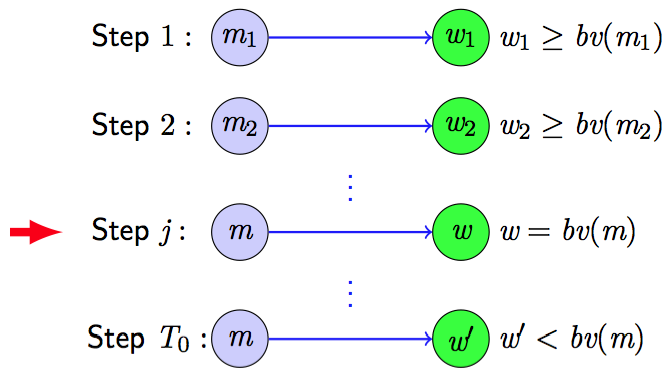
\includegraphics[width=2in]{L1-stablematchproofstep1.png}
 \end{figure}
 
\end{itemize}
} 

\frame{
\frametitle{Proof cont'd }
 \begin{itemize}
\item But $m$ finally didn't pair with $w$. Why? There are two cases: 
\begin{enumerate} 
 \item $m$ was rejected by $w$ directly: $w$ has already paired with $m'$ and in
her rank list,  $m'$ is better than $m$ (see left-hand panel).
 \item $m$ was accepted by $w$ but was dumped by $w$ afterwards: $m'$ is
proposing $w$ and and in her rank list, $m'$ is better than $m$ (see
right-hand panel).
\end{enumerate}
\begin{figure} 
 \begin{minipage}{0.45\textwidth}
  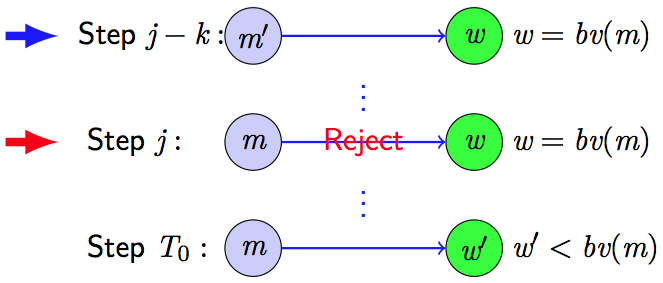
\includegraphics[width=1.8in]{L1-stablematchproofstep1case1.png}
 \end{minipage}
 \begin{minipage}{0.45\textwidth}
  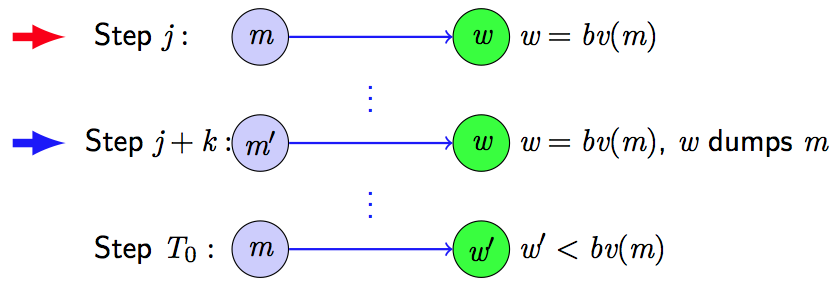
\includegraphics[width=2.3in]{L1-stablematchproofstep1case2.png}
 \end{minipage}
\end{figure}

\item In both cases, the following property holds: 
\begin{enumerate}
 \item For $w$: $w$ prefers $m'$ to $m$.
 \item For $m'$: $w\geq best\_valid(m')$ since $T_{0}$ is the first time that an ``unlucky'' proposal occurs.   
\end{enumerate}
\end{itemize} 
}

\frame{
\frametitle{Proof cont'd }
\begin{itemize}
 \item  The fact that $w$ is best valid partner of $m$ means that there exists a stable matching, denoted as $S'$, where $m$ pairs with $w$. Suppose that $m'$ pairs with $w''$ in $S'$. 
 
 \begin{figure}
\begin{tikzpicture}[scale=1., auto,swap]
   
        \foreach \pos/ \name in {{(0,1)/m},{(0,2)/m'}} 
        \node[vertex,fill=blue!20] (\name) at \pos{$\name$};

    \foreach \pos/ \name in {{(2.4,1)/w},{(2.4,2)/w''}} 
        \node[vertex,fill=green] (\name) at \pos {$\name$};
     
    % Connect vertices with edges and draw weights
    \foreach \source/ \dest/\weight in {m'/w''/{}, m/w/{} }
        \path[undirectededge] (\source) -- node[weight] {$\weight$} (\dest);

   \foreach \source/ \dest/\weight in {m'/w/{}}
        \path[undirectededge, red, dashed] (\source) -- node[weight] {$\weight$} (\dest);
%        
%\draw[ -latex, blue, line width=3pt ] (4.2, 1.5) -- (4.8, 1.5); 

 \node[above, color=black] at (1.2, 2.6) {Stable match $S'$}; 
 \node[right, color=black] at (2.8, 1) {$w=bv(m)$ }; 

      \end{tikzpicture}

\end{figure}


% \begin{figure}
%       \centering
%       \includegraphics[width=1.6in]{L1-stablematchproofstep2.eps}
% \end{figure}
 \item Then $m'-w$ should be an unstable pair. (Why?) \\
  \item A contradiction. In other words, unlucky proposals never occur in the ``propose-engage'' process, and any executions of the algorithm yields the same stable matching. 
\end{itemize}
}

\frame{
	\begin{block}{}
		Applications and awards
	\end{block}
}

\frame{
\frametitle{ Applications } 
	\begin{itemize}
	\item Assigning new doctors to hospitals;
	\item Assigning students to schools --- Public school systems in New York, Boston, Chicago and Denver use an algorithm based on his work to help assign students to schools.
	\item Finding kidney donors ---  {\it For example, a man needs a kidney, and his wife is willing to donate one of hers but she is not a match. Across the country there is a couple in the same position, and it turns out that the wives are a match for the husbands in the opposite couple. In this simple case, the two couples essentially barter their kidneys: Wife A gives her kidney to Husband B, and Wife B gives her kidney to Husband A. It is rare that two couples will serendipitously match each other’s kidney donation needs this way, and there are often more pairs of donor-recipients involved. Mr. Roth’s system helps find the most efficient exchange of organs so that the most patients can be saved with the fewest number of pairs involved in a given trade. }
	\end{itemize}
}
 
\frame{
\frametitle{ Nobel prize 2012 in Economic Sciences } 
 \begin{figure}
       \centering
       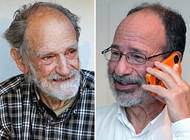
\includegraphics[width=1.05in]{Shapley-and-Roth.jpg}
       \caption{ {\small L. Shapley (left) and A. Roth (right)} }
 \end{figure}
{\small 
\begin{itemize}
	\item This year's Prize concerns a central economic problem: how to match different agents as well as possible. For example, students have to be matched with schools, and donors of human organs with patients in need of a transplant. How can such matching be accomplished as efficiently as possible? What methods are beneficial to what groups? 
	\item The prize rewards two scholars who have answered these questions on a journey from abstract theory on stable allocations to practical design of market institutions.
	The laureates’ breakthroughs involve figuring out how to properly assign people and things to stable matches when prices are not available to help buyers and sellers pair up.
\end{itemize}
}
}

\frame{
\frametitle{Nobel prize winner: Lloyd Shapley     } 
	\begin{itemize}
		\item {\bf Lloyd Shapley} used so-called cooperative game theory to study and compare different matching methods. A key issue is to ensure that a matching is stable in the sense that two agents cannot be found who would prefer each other over their current counterparts. Shapley and his colleagues derived specific methods – in particular, the so-called Gale-Shapley algorithm – that always ensure a stable matching. These methods also limit agents' motives for manipulating the matching process. Shapley was able to show how the specific design of a method may systematically benefit one or the other side of the market.
		\end{itemize}
}

\frame{
\frametitle{Nobel prize winner: Alvin Roth   } 
	\begin{itemize}
	\item {\bf Alvin Roth}  recognized that Shapley's theoretical results could clarify the functioning of important markets in practice. In a series of empirical studies, Roth and his colleagues demonstrated that stability is the key to understanding the success of particular market institutions. Roth was later able to substantiate this conclusion in systematic laboratory experiments. He also helped redesign existing institutions for matching new doctors with hospitals, students with schools, and organ donors with patients. These reforms are all based on the Gale-Shapley algorithm, along with modifications that take into account specific circumstances and ethical restrictions, such as the preclusion of side payments.
	\end{itemize}
} 

\frame{
\frametitle{ From theory to practice   } 
	\begin{itemize}
	\item 
Even though these two researchers worked independently of one another, the combination of Shapley's basic theory and Roth's empirical investigations, experiments and practical design has generated a flourishing field of research and improved the performance of many markets. This year's prize is awarded for an outstanding example of economic engineering.
	\end{itemize}
	\footnote{ These slides are excerpted from Nobleprize.org} 
}

\end{document}
